% This must be in the first 5 lines to tell arXiv to use pdfLaTeX, which is strongly recommended.
\pdfoutput=1
% In particular, the hyperref package requires pdfLaTeX in order to break URLs across lines.

\documentclass[11pt]{article}


\usepackage[preprint]{acl}

% style packages
\usepackage{times}
\usepackage{latexsym}
\usepackage[T1]{fontenc}
% This assumes your files are encoded as UTF8
\usepackage[utf8]{inputenc}
\usepackage{microtype}
\usepackage{inconsolata}


\usepackage{graphicx}
\usepackage{longtable}
\usepackage{array,etoolbox}
\usepackage{hyperref}
\usepackage{orcidlink}
\usepackage{acronym}
\usepackage{amsmath}
\usepackage{float}
\usepackage{algorithm}
\usepackage[noend]{algpseudocode}
\usepackage{enumitem}
\usepackage{amsfonts}
\usepackage{booktabs}

% table commands
\renewcommand{\arraystretch}{1.2}
% graphix commands
\graphicspath{ {./resources}  }


% links
\newcommand{\projectlink}{\footnote{\url{https://github.com/dimits-ts/synthetic_discussion_framework}}}
\newcommand{\analysislink}{\footnote{\url{https://github.com/dimits-ts/synthetic_moderation_experiments}}}
\newcommand{\datasetlink}{\footnote{\url{https://paperswithcode.com/dataset/vmd}}}
\newcommand{\textWarning}[1]{\begin{center}\textcolor{red}{\textbf{#1}}\end{center}}

% math
\DeclareMathOperator*{\argmax}{argmax} % thin space, limits underneath in displays

\title{Scalable Evaluation of Online Facilitation Strategies via Synthetic Simulations}
\author{
    Dimitris Tsirmpas \orcidlink{0000-0002-5675-3939}, Ion Androutsopoulos \orcidlink{0009-0000-2969-0509}, John Pavlopoulos \orcidlink{0000-0001-9188-7425} \\
    Dept.\ of Informatics, Athens University of Economics and Business, Greece and \\
    Archimedes, Athena Research Center, Greece \\
    \texttt{\{dim.tsirmpas,ion,annis\}@aueb.gr}
}
\date{February 2025}

\begin{document}

\maketitle

%\textWarning{Content warning: This paper contains samples of harmful text, including violent, toxic, controversial, and potentially illegal statements.}

% !TEX root = ../main.tex
%

\begin{abstract}
    Limited large-scale evaluations exist for online facilitation strategies due to significant costs associated with human involvement. An effective solution is synthetic discussion simulations using \acp{LLM} to create initial pilot experiments. We propose a simple and generalizable \ac{LLM}-driven methodology to prototype \ac{LLM} moderators, and produce high-quality synthetic data without human involvement. We use our methodology to test whether modern facilitation strategies can improve  the performance of \ac{LLM} facilitators. We find that, while \ac{LLM} facilitators significantly improve synthetic discussions, there is no evidence suggesting that the application of modern facilitation strategies leads to further improvements in discussion quality. Finally, we validate that each component of our methodology contributes meaningfully to high quality data via an ablation study,  we release an open-source framework, \syndisco\pip  which implements our methodology, and release \vmd a large, publicly available dataset containing \ac{LLM}-generated and annotated discussions from multiple open-source \acp{LLM}.\datasetlink
\end{abstract}


 


% !TEX root = ../main.tex
%
\section{Introduction}
\label{sec:introduction}

Research on conversational moderation/facilitation techniques (distinct from “content moderation”, which involves flagging and removing content) is crucial for adapting to evolving online environments, but lags significantly behind current demands \cite{seering_self_moderation, make_reddit_great}. A major challenge lies in the substantial costs required both in researching and moderating discussions, due to human participation \cite{rossi_2024}. Many platforms overcome this by outsourcing moderation to volunteers or users \cite{Matias2019TheCL, schaffner_community_guidelines}, while others turn to content moderation using traditional \ac{ML} models, which are not enough in practice \cite{horta_automated_moderation, schaffner_community_guidelines}. \acfp{LLM} have been hypothesized to be capable of conversational moderation and facilitation tasks \cite{small-polis-llm, korre2025evaluation}. While studies exist for simulating user interactions in social media \cite{park_simulacra, mou_2024, tornberg_2023, y_social, balog_2024}, and for using synthetic moderators \cite{kim_et_al_chatbot, cho-etal-2024-language}, none so far have combined the two approaches. 

\begin{figure}[hbt!]
	\centering
	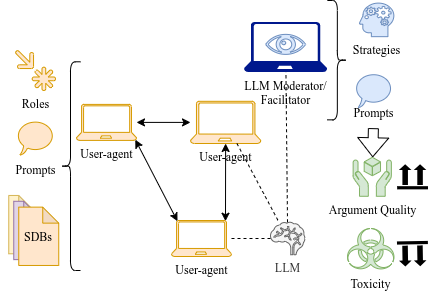
\includegraphics[width=\columnwidth]{research_goal.png}
	\caption{The \ac{LLM} user-agents conduct a discussion, while the \ac{LLM} moderator monitors and attempts to increase its quality. We need to design prompts and configurations for both.}
	\label{fig::goals}
\end{figure}


We propose a simple and generalizable approach using \ac{LLM}-driven synthetic experiments for online moderation research, enabling fast and inexpensive model “debugging” and parameter testing (e.g., selection of prompts, \ac{LLM} moderator instructions) without human involvement (Section \ref{sec:methodology}) (Fig. \ref{fig::goals}). We conduct an ablation study (Section \ref{ssec:results:ablation}), demonstrating that each step of our methodology meaningfully contributes to generating high-quality synthetic data, as well as examining the output of various \acp{LLM}. We do not make the claim that the behavior of \ac{LLM} user-agents is representative of human behavior, as this claim can be scarcely made in Social Science studies involving \ac{LLM} test subjects—we discuss this subject in depth in Section \ref{ssec:related:human-llm}. Using this methodology, we examine four \ac{LLM} moderation strategies based on current Social Science facilitation research (Section \ref{sec:experimental})
%: \ac{LLM} alignment guidelines \cite{collective_constitution}, prompts based on human facilitation guidelines \cite{Cornell_eRulemaking2017, dimitra-book} and our own prompt based on \ac{RL} (although we do not perform \ac{RL} in this paper). We 
and compare them with two baselines. We then evaluate these discussions using \ac{LLM} annotator-agents. We use open-source \acp{LLM} and include all relevant configurations in order to make our study as reproducible as possible (see Appendix \ref{ssec:appendix:annotation}, \ref{ssec:appendix:prompts}).


 Our analysis reveals two key findings (Section \ref{sec:results}): (1) the presence of \ac{LLM} moderators exhibited a positive and statistically significant influence on the quality of synthetic discussions and (2) current moderation strategies are often not enough to meaningfully outperform simple baselines. %However, besides helping in understanding the effect of prompts to \ac{LLM} moderators, the synthetic data presented in this paper can also be used to finetune them.

We also release “SynDisco”, an open-source Python framework for generating and evaluating synthetic discussions, along with the \acf{VMD}\datasetlink—a publicly available dataset comprising the evaluated discussions (Section \ref{sec:data-soft}). Finally, we outline the limitations (Section \ref{sec:limitations}) and ethical considerations (Section \ref{sec:ethical}) of our work.
% !TEX root = ../main.tex
%

\section{Related Work}


\subsection{Synthetic discussions}

\ac{LLM} agents talking with each other has been an active area of research outside the context of discussion simulation. The term “\ac{LLM} self-talk” is usually used in this case, a term adapted from “self-play” in \ac{RL} \citep{cheng2024selfplayingadversariallanguagegame}). For instance, researchers have experimented with using self-talk for reinforcing \acp{LLM} against jailbreaking \cite{liu2024largelanguagemodelsagents, cheng2024selfplayingadversariallanguagegame, zheng2024optimalllmalignmentsusing}, for \ac{LLM} alignment \cite{Bai2022ConstitutionalAH, collective_constitution}, and self-refinement in general \cite{Madaan2023SelfRefineIR, lambert2024} by pitting the model against itself. \citet{ulmer2024} give their \ac{LLM} agents distinct roles in a conversational setting and demonstrate that \ac{LLM} self-talk can occasionally produce high-quality, convincing discussions. These discussions can be used to further finetune the model.  \citet{abdelnabi_negotiations} show that \acp{LLM} can execute (to some extent) social strategies in discussions in order to achieve long-term goals. An example is a negotiation where an environmentalist \ac{LLM} agent may be stoking disagreement between other agents, in order to eventually sabotage the negotiations for the creation of a new factory.


\subsection{Replicating human behavior with LLMs}

Studies demonstrate that while \acp{LLM} can not fully replicate human behavior, they approximate it to a limited extent. \citet{hewitt2024predicting} recommend employing \acp{LLM}s in social science experiments for minority groups, particularly pilot studies, but highlight limitations including low variance, model bias, and challenges in encoding all participant details into prompts. \citet{park2024generativeagentsimulations1000} reveal that substituting \acp{SDB} with interview-based information enhances their authenticity. However, their approach relies on extensive human interviews and computational resources.

\acp{LLM} can also simulate human behavior within communities. \citet{park_simulacra} use a single \ac{LLM} with \ac{SDB} prompting to generate entire Reddit communities, producing synthetic discussions indistinguishable from real ones. \citet{Park2023GenerativeAI} create an interactive in-game world where \ac{LLM}-controlled \acp{NPC} engage with players, the environment, and each other, displaying complex social behavior like information sharing and event planning. However, they note that these agents tend to be “too agreeable”, likely due to alignment artifacts.

% !TEX root = ../main.tex
%

\section{Methodology}
\label{sec:methodology}

\subsection{Defining Synthetic Discussions}

Let $U$ be the set of users participating in discussions and $M$ the set of moderators, where $M \cap U = \emptyset$. We define a conversation $d$ of $\lvert d \rvert$ comments\footnote{Also referred to as “dialogue turns” in some publications.} $c(d, i)$ as an ordered set:
\begin{equation}
    d = \{c(d, 1), c(d, 2), \ldots, c(d, \lvert d \rvert)\}
\end{equation}


Next, we define a turn-taking function $u: D  \times \mathbb{N} \rightarrow U \cup M$ mapping a comment in the $i$-th turn of a discussion $d \in D$ to an arbitrary user in $U$, or moderator in $M$. In real discussions, $u$ is not strictly defined, since which user responds to each comment can not be reliably determined. However, in a synthetic environment $u$ can be made deterministic (see the function formulation at Equation \ref{eq:turn_taking} in Section \ref{ssec:experimental:discussions} for an example).

In our case, all comments are synthetic, hence, a comment $c$ in a discussion $d \in D$, at the $i$-th turn is defined recursively as:

\begin{equation}
\begin{split}
    c(d, i) = & LLM([c(d, j)]^{i-1}_{j=max(1, i-h)};\\
    &\phi(u(d, i)))
\end{split}
\end{equation}

\noindent where $[\cdot]$ is string concatenation and $h$ is the context length of the \ac{LLM} user-agent (how many past comments they can “remember”) and $\phi: U \times M \rightarrow s$ is a function mapping a user $u$ to their instruction prompt $s$.

Our methodology thus assumes that the contents of any synthetic discussion are dependent on the following parameters:
\begin{itemize}[noitemsep]
    \item The underlying model ($LLM(\cdot)$)
    \item The turn-taking function $u$
    \item The prompting function $\phi$
\end{itemize}


\subsection{Gauging Diversity}
\label{ssec:methodology:evaluating}

One simple metric that distinguishes between LLM generated and human texts, is the one presented in \citet{ulmer2024}. In their work, the authors use average pairwise F1 ROUGE-L scores \cite{lin-2004-rouge} to gauge diversity in synthetic discussions. This is built on the observation that a common shortcoming of completely synthetic discussions is word repetition; either because the discussion does not meaningfully advance, or because the discussion collapses (and the models keep repeating the same words/phrases). The score is computed by computing the individual F1 ROUGE-L scores for each comment in the discussion with all the rest, then averaging them. A larger ROUGE-L score indicates less variance in the discussion. The equation itself can be written as:

\small
\begin{equation}
\label{eq:variety}
    div(d) = \frac{1}{N(N-1)} \sum_{i=1}^N \sum_{j=1, j \neq i}^N F1(c(i, d), c(j, d))
\end{equation}
\normalsize
\section{Experimental Setup}
\label{sec:experimental}

\subsection{Facilitation Strategies}
\label{ssec:experimental:strategies}

We test four different facilitation strategies, along with two common-place strategies for discussion facilitation. Note that the process of turning sometimes extensive documents into short prompts, necessitated by open-source LLMs, is necessarily imperfect. We leave the optimal derivation of strategy prompts to future work.

\begin{enumerate}[nosep, noitemsep]
    \item \textbf{\strategynomod}: A \emph{common} strategy where no facilitator is present.

    \item \textbf{\strategynoinstr}: A \emph{common} strategy where a LLM facilitator is present, but is provided only with basic instructions. Example: “You are a moderator, keep the discussion civil”.

    \item \textbf{\strategyrules}: A \emph{real-life} strategy where the prompt is adapted from LLM alignment guidelines \cite{collective_constitution}. These guidelines were selected to be as unanimously agreed upon across various human groups. They thus provide a set of rules to uphold, without specifying \emph{how} to uphold them (e.g, “Be fair and impartial, assist users, don't spread misinformation”).

    \item \textbf{\strategyregroom}: A \emph{real-life} strategy based on guidelines given to human facilitators of the ``Regulation Room'' platform \citep{Cornell_eRulemaking2017}. The instructions are typical of online moderation. Example: ``Stick to a maximum of two questions, use simple and clear language, deal with off-topic comments''.

    \item \textbf{\strategyconstrcomm}: A \emph{real-life} strategy based on the human facilitation guidelines used by the MIT Center for Constructive Communications \cite{dimitra-book}. It approaches facilitation from a more personalized and indirect angle, forbidding facilitators from directly providing opinions or directions. Example: ``Do not make decisions, be a guide, provide explanations''.
    
    \item \textbf{\strategymodgame}: Our proposed \emph{experimental} strategy, inspired by \citet{abdelnabi_negotiations} (see \S\ref{ssec:related:discussions}). Instructions are formulated as a game, where the facilitator LLM tries to maximize their scores by arriving at specific outcomes. No actual score is being kept; they exist to act as indications for how desirable an outcome is. The other participants are not provided with scores, nor are they aware of the game rules. Example: ``User is toxic: $-5$ points, User corrects behavior: $+10$ points''.
\end{enumerate}


\subsection{Synthetic Discussion Generation}
\label{ssec:appendix:discussion}

An overview of how the experiments are generated can be found in Algorithm~\ref{alg:exp_generation}. We provide our framework with a set of starting opinions (``seed opinions'') and SDBs. We then run $N_d=8$ discussions for each pair of facilitation strategies $S$ and model. Synthetic generation is then handled as described in \S\ref{sec:methodology}. 

\begin{algorithm}[t]
	\caption{Synthetic discussion setup generation}
	\label{alg:exp_generation}
	\hspace*{\algorithmicindent} \textbf{Input:} 
	\begin{itemize}[noitemsep, nosep]
		\item User SDBs $\Theta = \{\theta_1, \dots, \theta_{30}\}$
		\item Moderator SDB = $\theta_{mod}$
		\item Strategies $S = \{s_1, \ldots, s_6\}$
		\item Seed opinions $O = \{o_1, \ldots, o_7\}$
		\item LLMs = $\{llm_1, llm_2, llm_3\}$
	\end{itemize}
	\hspace*{\algorithmicindent} \textbf{Output:} Set of discussions $D$
	\begin{algorithmic}[1]
		\State $D = \{\}$
		\For{$llm \in LLMs$}
		\For{$s \in S$}
		\For{$i = 1, 2, \ldots, N_d$}
		\State $\hat{\Theta} = $ \Call{RandomSample}{$\Theta$, 7}
		\State $U =$  \Call{Actors}{llm, $\hat{\Theta}$}
		\State $m = $ \Call{Actors}{llm, $\{[\theta_{mod}, s]\}$}
		\State $o = $ \Call{RandomSample}{$O$, 1}
		\State $d =$ \{users: $U$, mod: $m$, topic: $o$\}
		\State $D = D \cup d$
		\EndFor
		\EndFor
		\EndFor
		\State \Return $D$
	\end{algorithmic}
\end{algorithm}


\subsection{Evaluation}
\label{ssec:experimental:evaluation}

In our study, we use \emph{toxicity} as a proxy for discussion quality, since it can inhibit online and deliberative discussions \citep{dekock2022disagree, XiaToxicity}\footnote{We note that this is not always true \citep{Avalle2024PersistentIP}.}. We use ten LLM annotator-agents controlled by a model already used in prior work (LLaMa3.1 70B) \cite{kang-qian-2024-implanting} (\S\ref{ssec:experimental:evaluation}), as LLMs are reliable for toxicity detection \citep{kang-qian-2024-implanting, Wang2022ToxicityDW, anjum2024hate}.

In order to gauge the quality of our synthetic discussions, since we can not reliably measure ``realism'' \cite{rossi_2024}, we use the ``diversity'' metric \citep{ulmer2024}. Low diversity points to pathological problems (e.g., LLMs repeating previous comments). On the other hand, extremely high diversity may point to a lack of interaction between participants; a discussion in which participants engage with each other will feature some lexical overlap (e.g., common terms, paraphrasing points of other participants). We compare the distribution of diversity scores for synthetic discussions with that measured on sampled human discussions. This allows us to estimate the extent to which synthetic discussions approximate real-world content variety and participant interaction. 

We note again that these metrics are better interpreted as heuristics of actual discussion and synthetic data quality respectively. More research is needed w.r.t. reliable and generalizable quality metrics.


\subsection{Technical Details}
\label{ssec:experimental:setup}

We use three instruction-tuned, open-source models: LLaMa 3.2 (70B), Qwen2.5 (33B),  Mistral Nemo (12B), quantized to 4 bits. All the experiments were collectively completed within four weeks of computational time, using two Quadro RTX 6000 GPUs. The process of generating discussion setups is detailed in \S\ref{ssec:appendix:discussion}. The execution script is available in the project's repository.\analysislink 
% !TEX root = ../main.tex
%

\section{Results}
\label{sec:results}


\subsection{Main findings}
\label{ssec:results:main}

\paragraph{Finding 1: LLM facilitators significantly improve synthetic discussions over time by restraining the toxicity of all participants---including trolls.} As illustrated in Fig.~\ref{fig:toxicity_stats}, unmoderated discussions tend to display significantly higher levels of toxicity. A linear regression analysis of toxicity over time ($Adj. R^2 = 0.413$) reveals that trolls begin with markedly higher toxicity—on average $1.3288$ points above neutral users and $1.3112$ above community veterans ($p < .000$). However, their toxicity decreases by an average of $\minus0.0125$ points per turn ($p = 0.003$). This trend is even more pronounced for neutral participants and community veterans, whose toxicity drops by $\minus0.0225$ ($p < .000$) and $\minus0.0350$ ($p < .000$) points per turn, respectively. These findings indicate that LLM facilitators are effective in guiding conversations toward reduced toxicity over time, despite the lack of punitive measures. While trolls are less responsive, they still show a clear reduction in toxic behavior as the discussion progresses.

\begin{figure}
	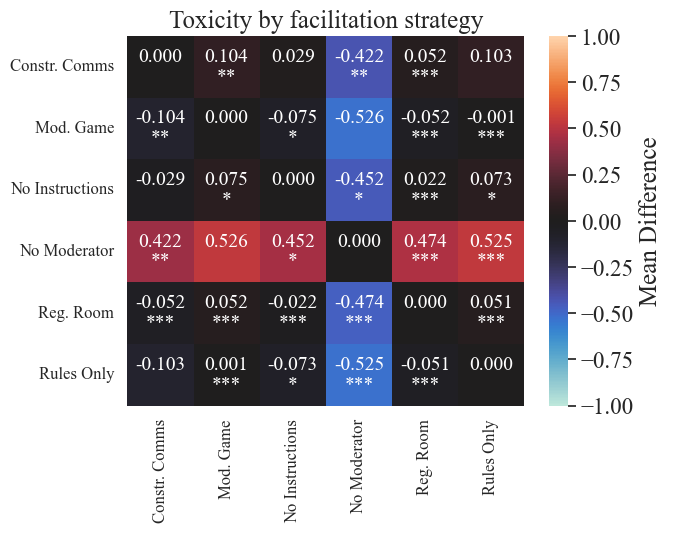
\includegraphics[width=\linewidth]{toxicity_stats.png}
	\centering
	\caption{Difference in average toxicity levels for comments following pairs of facilitation strategies. Red cells ($x>0$) indicate that the strategy on the left performs worse than the one on the bottom, for an average of $x$ points in a scale of 1-5. Conversely for blue ($x<0$) cells. White cells denote minute changes. Asterisks derived from pairwise Student-t tests (\asterisknote). The large size of our dataset allows using parametric tests.}
	\label{fig:toxicity_stats}
\end{figure}

\paragraph{Finding 2: More elaborate facilitation strategies fail to decrease toxicity.}
Strategies such as \emph{\strategyregroom}, \emph{\strategyconstrcomm}, and our proposed \emph{\strategymodgame} significantly reduce comment toxicity compared to \emph{unmoderated} discussions, with their effectiveness increasing over time (Table~\ref{tab:toxicity}). However, these more elaborate facilitation approaches do not consistently outperform the simpler \emph{\strategynoinstr} strategy overall (Fig.~\ref{fig:toxicity_stats}). This suggests that out-of-the-box LLMs may struggle to meaningfully incorporate complex instructions—a limitation noted in prior work \cite{cho-etal-2024-language}. While the real-life strategies show a slight edge over time compared to \emph{\strategynoinstr}, the observed long-term gains are modest and not qualitatively significant in the broader context.

\begin{table}[t]
	\centering
	\begin{tabular}{p{5cm} p{1.5cm}}
		\toprule
		\textbf{Variable} & \textbf{Toxicity} \\
		\midrule
		Intercept & 2.164\textsuperscript{***} \\
		\strategynoinstr & -0.426\textsuperscript{***} \\
		\strategymodgame & -0.435\textsuperscript{***} \\
		\strategyrules & -0.461\textsuperscript{***} \\
		\strategyregroom & -0.277\textsuperscript{***} \\
		\strategyconstrcomm & -0.230\textsuperscript{***} \\
		time & -0.012\textsuperscript{**} \\
		\strategynoinstr$\times$time & -0.003 \\
		\strategymodgame$\times$time & -0.011\textsuperscript{*} \\
		\strategyrules$\times$time & -0.008 \\
		\strategyregroom$\times$time & -0.023\textsuperscript{***} \\
		\strategyconstrcomm$\times$time & -0.023\textsuperscript{***} \\
		\bottomrule
	\end{tabular}
	\small
	\asterisknote
	\normalsize
	\caption{OLS regression coefficients for toxicity on the non-facilitator comments ($Adj. R^2=0.054$). Reference factor is \textit{\strategynomod}. All strategies outperform \textit{\strategynomod} in general. The \textit{\strategyregroom} and \textit{\strategyconstrcomm} real-life strategies additionally show improvements over time compared to \textit{\strategynomod}.}
	\label{tab:toxicity}
\end{table}


\paragraph{Finding 3: LLM facilitators choose to intervene far too frequently, which is tolerated by the other participants.} Fig.~\ref{fig:intervention_count} demonstrates that LLM facilitators intervene at almost any opportunity, even though they are instructed to only do so when necessary. This confirms that LLMs generally can not decide not to speak even when instructed to do so  (\S\ref{ssec:methodology:turn}). To our knowledge, this has not been reported in relevant literature, and \emph{is an example of ``debugging'' problems with LLMs} --- a core motivation of our work.

Additionally, a qualitative look through the dataset reveals that LLM user-agents exhibit atypical tolerance for excessive facilitator interventions. Humans in contrast, typically become irritated and more toxic after repeated, unneeded interventions \citep{schaffner_community_guidelines, make_reddit_great, proactive_moderation, cresci_pesonalized_interventions}. This is likely another artifact caused by alignment procedures, making LLMs too agreeable \citep{park2023game, anthis_2025}.

\begin{figure}[t]
	\centering
	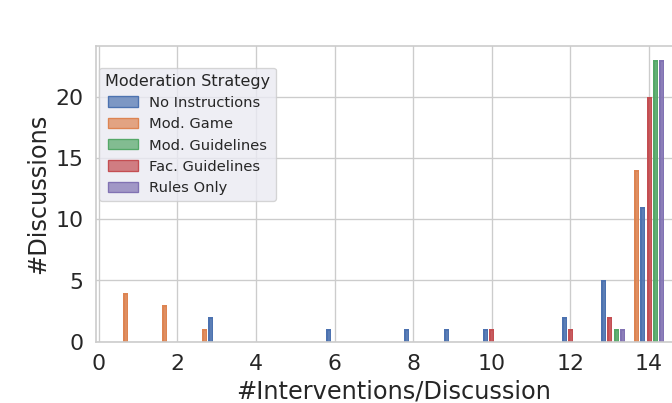
\includegraphics[width=\columnwidth]{intervention_count.png}
	\caption{Histogram of interventions by LLM facilitators per strategy used.}
	\label{fig:intervention_count}
\end{figure}


\subsection{Ablation Study}
\label{ssec:results:ablation}

\begin{figure}[t]
	\centering
	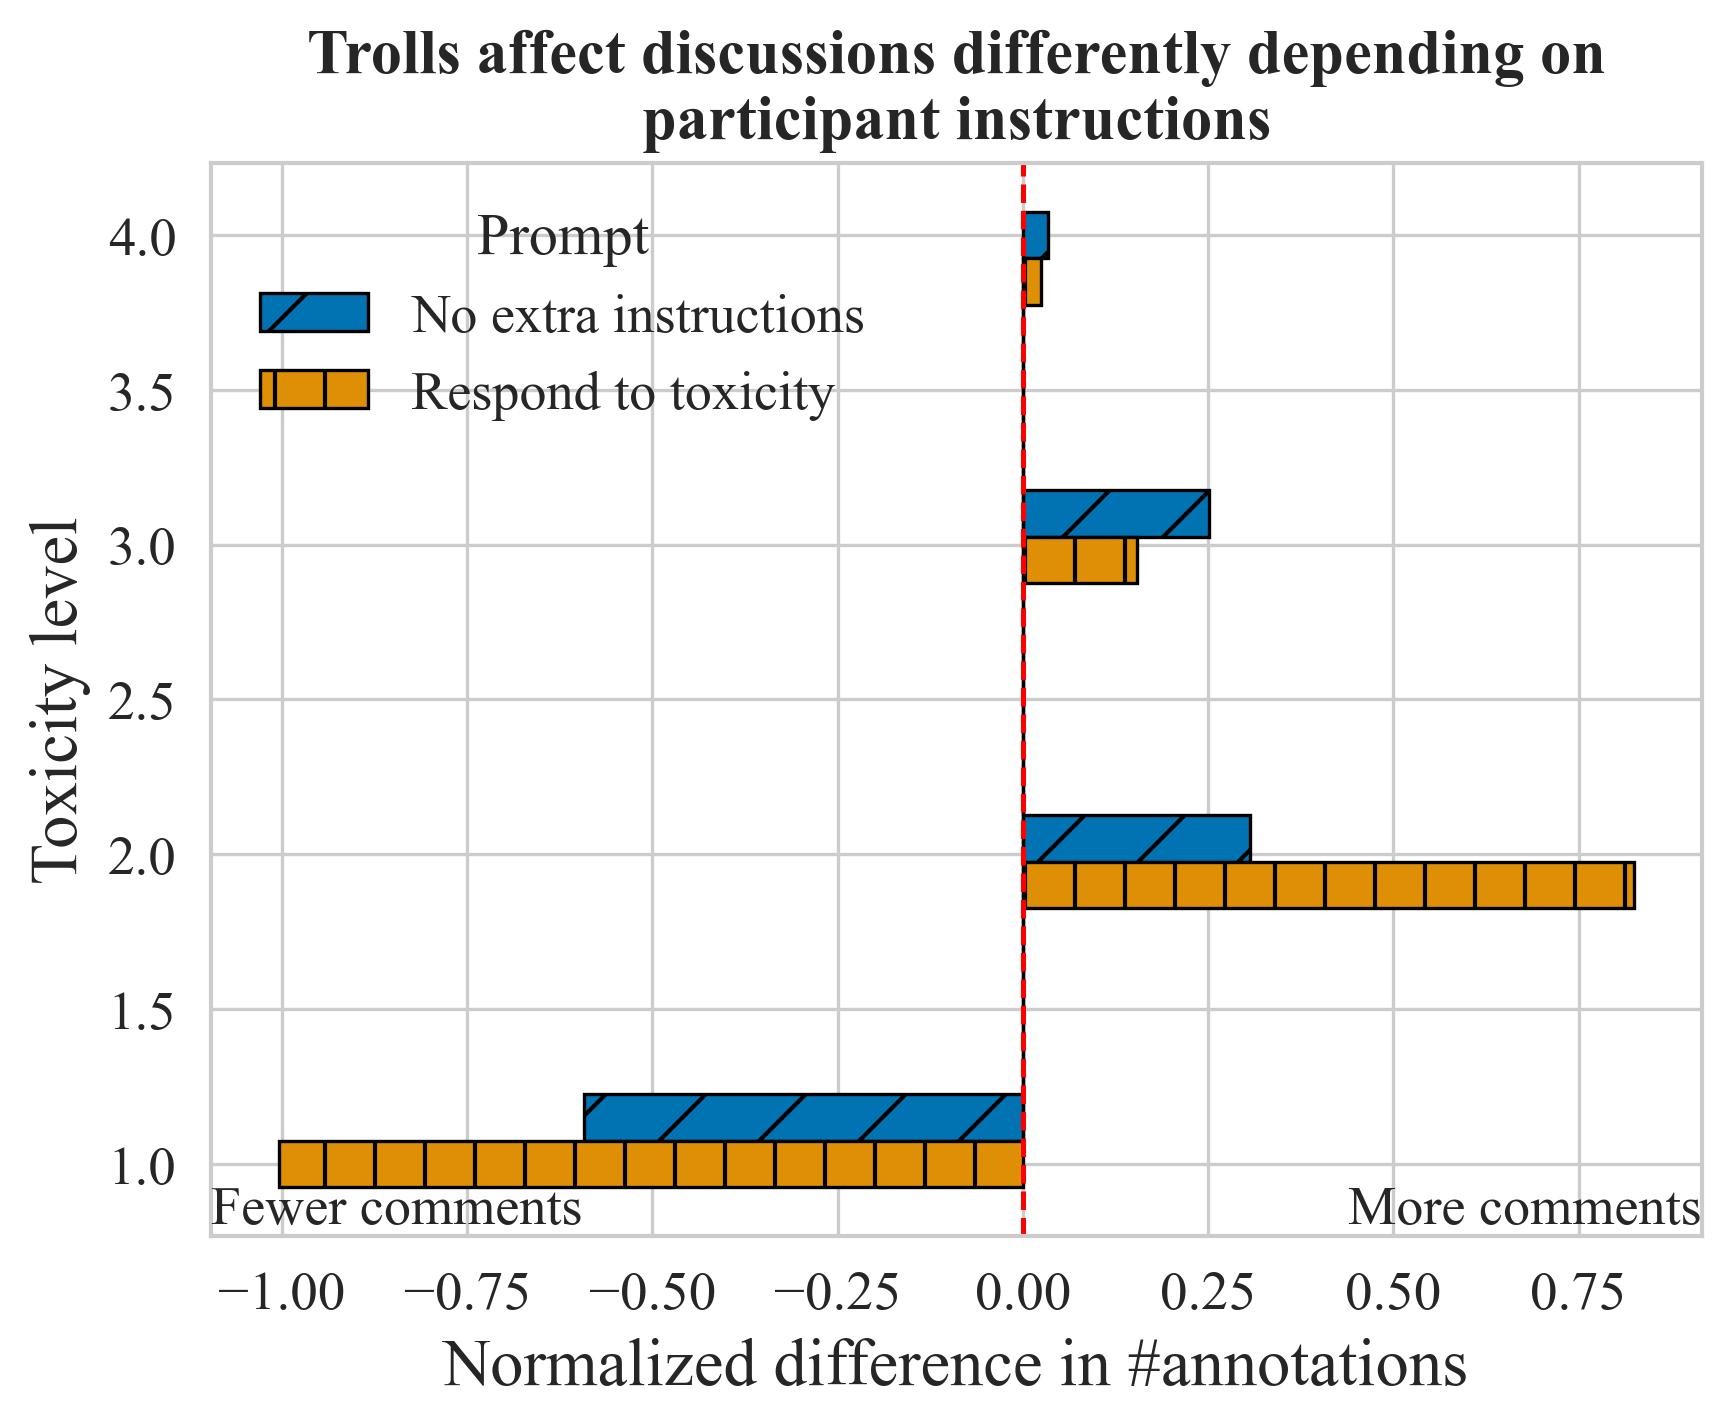
\includegraphics[width=0.8\linewidth]{toxicity_trolls.png}
	\caption{Non-troll toxicity levels in discussions with and without trolls. There is a significant uptick on the number of ``somewhat toxic" ($Toxicity=2$) comments when the participants are primed to respond to toxic comments (lower bars).}
	\label{fig:toxicity_trolls}
\end{figure}

\begin{figure*}[t]
	\begin{subfigure}{0.32\linewidth}
		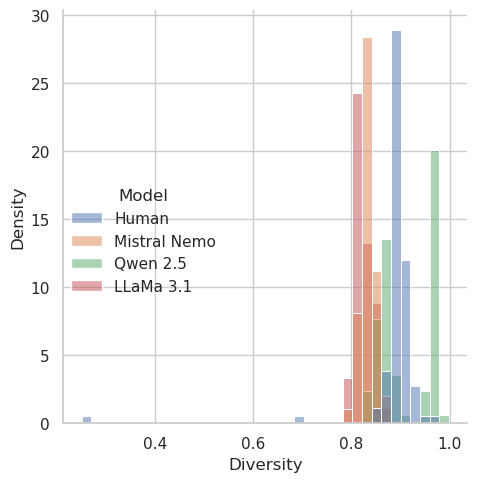
\includegraphics[width=\textwidth]{rougel_model.png}
		\caption{Model}
		\label{fig:rougel_model}
	\end{subfigure}%
	\hfill
	\begin{subfigure}{0.32\linewidth}
		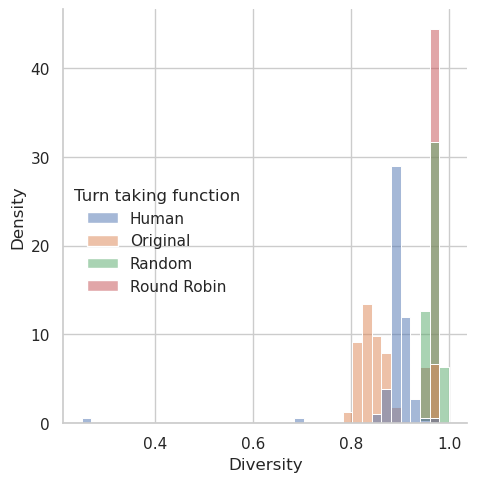
\includegraphics[width=\textwidth]{rougel_turns.png}
		\caption{Turn-taking function}
		\label{fig:rougel_turns}
	\end{subfigure}%
	\hfill
	\begin{subfigure}{0.32\linewidth}
		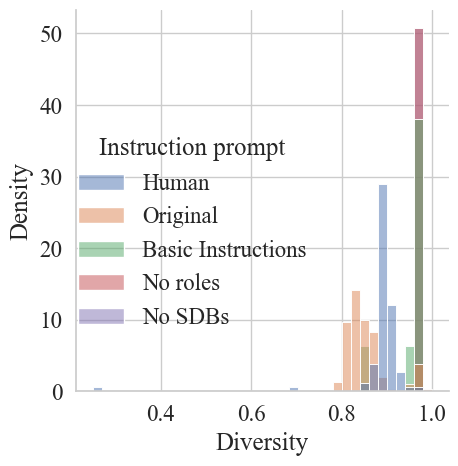
\includegraphics[width=\textwidth]{rougel_prompts.png}
		\caption{Instruction prompt}
		\label{fig:rougel_prompts}
	\end{subfigure}%
	
	\caption{Diversity (\S\ref{ssec:related:quality}) distribution for each discussion by LLM (\S\ref{ssec:experimental:setup}), turn-taking function $t$ (\S\ref{ssec:methodology:turn}), and prompting function $\phi$ used (\S\ref{ssec:methodology:prompts-instructions}). Comparison with the CeRI Regulation Room dataset (``Human''). Note that the x-axis starts from $0.6$.}
	\label{fig:diversity}
\end{figure*}

We generate eight synthetic discussions per ablation experiment, using a single model (Qwen 2.5). We compare the diversity (cf. \S\ref{ssec:related:quality}, \S\ref{ssec:experimental:evaluation}) of these discussions with ones from the CeRI “Regulation Room” dataset as well as the discussions from our broader synthetic dataset.\footnote{Disclaimer: Any opinions, findings, and conclusions or recommendations expressed in this material are those of the author(s) and do not necessarily reflect the views of the CeRI.} We pick this dataset because it is publicly available and comprised of facilitated online human discussions on ten diverse topics.

\paragraph{Each component of our methodology surpasses baselines in data quality} We compare our turn-taking function (\S\ref{ssec:methodology:turn}) to two baselines: Round Robin (participants speaking one after the other, then repeating) and Random Selection (uniformly sampling another participant each turn). Fig.~\ref{fig:rougel_turns} demonstrates that although all distributions diverge from the blue—human—distribution, our function is the only one not exhibiting extremely high diversity (i.e., very limited participant interaction \S\ref{ssec:experimental:evaluation}). Fig.~\ref{fig:rougel_prompts} illustrates that each individual prompting function (SDBs, roles, and instruction prompts) results in diversity scores more closely aligned with human discussions.

\paragraph{Larger models do not lead to more high-quality discussions.} As shown in Fig.~\ref{fig:rougel_model}, Qwen demonstrated the highest diversity among the evaluated models, indicating limited participant interaction (\S\ref{ssec:related:quality}), followed by Mistral Nemo and LLaMa. However, none of the models closely matched the diversity observed in human discussions. 

\paragraph{Specialized instruction prompts are essential for eliciting toxic behavior in instruction-tuned LLMs.} Our instruction prompt for the participants (\S\ref{ssec:methodology:prompts-instructions}) incentivizes them to react to toxic behavior. Indeed, inserting “troll” participants to discussions, leads to more intense toxicity among \emph{other} participants \emph{only if we instruct participants to react to toxic posts} (Fig.~\ref{fig:toxicity_trolls}). 

	
\section{Datasets \& Software}

We introduce SynDisco, an open-source, lightweight, purpose-built framework for managing, annotating, and generating synthetic discussions. Key features include: 
\begin{itemize}[nosep, noitemsep]
    \item  Three core functions: discussion management, synthetic annotation, and mass generation of randomized discussion and annotation tasks.
    \item  Built-in fault tolerance (automated recovery and intermittent saving) and file logging to support extended experiments.
    \item Easy installation via PIP (\texttt{pip install syndisco}).
\end{itemize}     

% !TEX root = ../main.tex
%

We also release \vmd\datasetlink a dataset of synthetic discussions annotated by LLMs. It can serve for finetuning facilitator LLMs. We note that, as is the case with most synthetic datasets \citep{ulmer2024}, the data may need to be filtered to derive only high-quality samples. In our case this would necessitate filtering out discussions with constant facilitator interventions or low/extremely high diversity scores. However, the data can be scaled accordingly, due to the low computational cost of our methodology.

 The supplementary ablation dataset, as well as the code for the analysis and the graphs present in this paper, can be found in the project repository\analysislink. The dataset is licensed under a CC BY-SA license, and the software under GPLv3. \textbf{Warning: The datasets by their nature contain offensive and hateful speech.}
% !TEX root = ../main.tex
%
\section{Conclusions \& Future Work}

Our study is the first to apply synthetic data generation to the field of online discussion moderation/facilitation. We propose a simple and generalizable methodology, which enables researchers to inexpensively conduct pilot online moderation experiments using exclusively synthetic \ac{LLM} user-agents. We also conduct an ablation study to demonstrate that each component of our methodology meaningfully results in higher-quality synthetic data.

We create an open-source Python Framework \syndisco that applies this methodology to hundreds of experiments, which we use to create and publish a large-scale synthetic dataset (\vmd). Using this dataset, we compare the effectiveness of numerous moderation strategies and baselines  for \ac{LLM} moderators, elicited from current conversational moderation research. We demonstrate that (1) \ac{LLM} moderators significantly improve the quality of synthetic discussions and (2) established human moderation/facilitation guidelines often do not surpass simple baselines with regard to toxicity and \ac{AQ}. We hope that the methodology, synthetic dataset, and software presented in this paper can help research in the domain of \ac{LLM}-based moderation, and that the data presented in this paper can help finetune models for online moderation.

% !TEX root = ../main.tex
%
\section{Discussion}
\paragraph{Future work}Future work should identify additional quality metrics to evaluate synthetic data, and discussion quality. The latter can then be used to examine the applicability of our findings obtained regarding optimal facilitation strategies, to discussions involving humans. It would also be interesting to explore how to more effectively prompt LLMs with complex facilitation strategies, or alternative formulations of our methodology, as described in this paper.
% !TEX root = ../main.tex
%
\section{Limitations} 
\label{sec:limitations}

Our experimental setup makes certain assumptions that may affect the generalizability of our findings. Principally, we investigate the effects of only three \acp{LLM}, we assume that at most one moderator is present in each simulated discussion, and our turn-taking algorithm does not account for contextual factors such as relevance or emotional engagement, which are critical in human discussions. Our study also does not account for meta-knowledge available to participants, as human users would likely behave differently when faced with a synthetic moderator compared to a human one. Lastly, our methodology does not attempt to simulate algorithmic recommendation systems, which would realistically play a role in the context of social media discussions.

Without conducting a large-scale human correlation study comparing synthetic and human-mediated discussions, we cannot fully evaluate the realism of our generated discussions. Furthermore, our analysis relies on annotations provided by \ac{LLM} agents, which introduces potential biases inherent to these models. Without empirical validation through extensive human correlation studies, we can not be certain about our evaluations of both the realism and the quality of synthetic discussions.
% !TEX root = ../main.tex
%
\paragraph{Ethical considerations} 
Synthetic discussions involving LLMs could be exploited by malicious actors to train them at performing unethical tasks \cite{majumdar_2024_nefarious, MARULLI20245340, li_2025_vulnerable}, although ongoing research is addressing these vulnerabilities \cite{wang_2025_risk}. Furthermore, the use of LLMs inherently risks skewing moderation systems towards the predominant demographics best represented in their training data. SDB prompts are a necessary but insufficient step towards avoiding this \cite{rossi_2024, anthis_2025, burton2024large}.

\paragraph{AI use statement} LLMs were used solely for styling and text corrections in this document. They were also partially used for generating framework documentation, and code for some of the presented graphs. All such changes and additions have been checked by the authors.

% !TEX root = ../main.tex
%
\section*{Acknowledgements}

Special thanks to our colleague, Katerina Korre, for providing extensive feedback on an earlier draft.

We have used small, open source LLMs (principally LLaMa-8b and Mistral Nemo) to help in small style changes throughout this paper. We also used them in conjunction with a GPT-4 model \cite{openai2024gpt4technicalreport} to write initial documentation for our framework, as well as to generate some of the code for the plots and the analysis presented in this paper. 

This work has been partially supported by project MIS 5154714 of the National Recovery and Resilience Plan Greece 2.0 funded by the European Union under the NextGenerationEU Program.

\bibliography{refs}
\appendix
\section{Appendix}
\label{sec:appendix}

\subsection{Acronyms Used}

\begin{acronym}[WWW] % Give the longest label here so that the list is nicely aligned
    \ifthenelse{\boolean{review}}
        {}
        {\acro{VMD}{Virtual Moderation Dataset}}
    
	\acro{LLM}{Large Language Model}
	%\acro{NPC}{Non-Playable Character}
	\acro{ML}{Machine Learning}
	\acro{RL}{Reinforcement Learning}
	\acro{SDB}{SocioDemographic Background}
    \acro{AQ}{Argument Quality}
    %\acro{IR}{Information Retrieval}
    %\acro{NLP}{Natural Language Processing}
    \acro{CeRI}{Cornell e-Rulemaking Initiative}
    \acro{nDFU}{normalized Distance From Unimodality}
    \acro{OLS}{Ordinary Least Squares}
    \acro{GLP}{GNU General Public License}
\end{acronym}


\subsection{Synthetic Discussion Generation}
\label{ssec:appendix:discussion}

An overview of how the experiments are generated can be found in Algorithm~\ref{alg:exp_generation}. Each discussion is run according to Eq.~\ref{eq:comment} in Section~\ref{ssec:methodology:discussions}.

\begin{algorithm}[t]
\caption{Synthetic discussion generation}
\label{alg:exp_generation}
\hspace*{\algorithmicindent} \textbf{Input:} 
         \begin{itemize}[noitemsep, nosep]
             \item User \acsp{SDB} $\Theta = \{\theta_1, \dots, \theta_{30}\}$
             \item Moderator \acs{SDB} = $\theta_{mod}$
             \item Mod. strategies $S = \{s_1, \ldots, s_6\}$
             \item Seed opinions $O = \{o_1, \ldots, o_7\}$
             \item \acp{LLM} = $\{llm_1, llm_2, llm_3\}$
         \end{itemize}
         \hspace*{\algorithmicindent} \textbf{Output:} Set of discussions $D$
\begin{algorithmic}[1]
    \State $D = \{\}$
    \For{$llm \in LLMs$}
        \For{$s \in S$}
            \For{$i = 1, 2, \ldots, n_{discussions}$}
                \State $\hat{\Theta} = $ \Call{RandomSample}{$\Theta$, 7}
                \State $U =$  \Call{Actors}{llm, $\hat{\Theta}$}
                \State $m = $ \Call{Actors}{llm, $\{[\theta_{mod}, s]\}$}
                \State $o = $ \Call{RandomSample}{$O$, 1}
                \State $d =$ \{users: $U$, mod: $m$, topic: $o$\}
                \State $D = D \cup d$
            \EndFor
        \EndFor
    \EndFor
    \State \Return $D$
\end{algorithmic}
\end{algorithm}


\subsection{Synthetic Annotation}
\label{ssec:appendix:annotation}

\subsubsection{Investigating Argument Quality}

While toxicity is a reliable and important metric, we can investigate other discussion quality dimensions, such as \ac{AQ}. \ac{AQ} is an important metric, frequently studied in the field of online facilitation \cite{argyle2023, schroeder-etal-2024-fora, falk-etal-2024-moderation, falk-etal-2021-predicting} and which can be correlated with toxicity \cite{chang-danescu-niculescu-mizil-2019-trouble}. However, it is also vague as a term; \citet{wachsmuth-etal-2017-computational} provide a definition comprised of logical, rhetorical, and dialectical dimensions, although other dimensions have also been proposed \cite{habernal-gurevych-2016-argument, persing-ng-2015-modeling}. Indeed, determining \ac{AQ} is a difficult task, since even humans disagree on what constitutes a ``good argument” \cite{wachsmuth-etal-2017-computational, argyle2023}.

Most findings w.r.t. toxicity are mirrored for \ac{AQ}. Fig.~\ref{fig:aq_stats} demonstrates that the presence of an \ac{LLM} facilitator qualitatively improves the \ac{AQ} of synthetic discussions, although to a lesser extent when compared with toxicity (c.f. Fig.~\ref{fig:toxicity_stats}). Similarly, there is no qualitative, observed improvement when advanced facilitation strategies are used (Fig.~\ref{fig:aq_stats}). \ac{LLM} users also show worse \ac{AQ} in the presence of trolls, when we use our specialized instruction prompt. Contrary to toxicity, the presence of \ac{LLM} facilitators does not seem to improve \ac{AQ} over time, as demonstrated in Table~\ref{tab:argq}.

\begin{figure}
	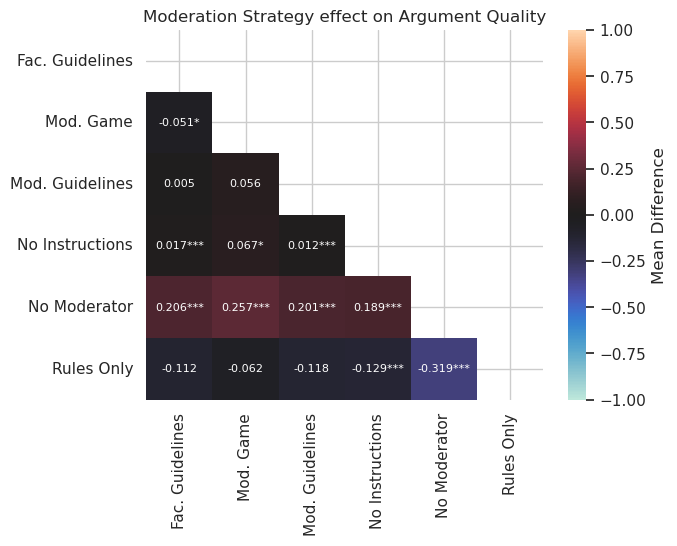
\includegraphics[width=\linewidth]{resources/argumentq_stats.png}
	\centering
	\caption{Mean difference of \ac{AQ} between pairs of facilitation strategies. For ease of comparison we follow the same scale and direction for \ac{AQ} as with toxicity: when the value of a cell at row $i$ and column $j$ is $x$, strategy $i$ leads to overall  worse ($x>0$), or better ($x<0$) \ac{AQ} compared to $j$ for an average of $x$ points in a scale of $1-5$. For each comparison, we use a pairwise Student t-test; p-values are shown as asterisks (\asterisknote).}
	\label{fig:aq_stats}
\end{figure}


\begin{table}
	\centering
	\begin{tabular}{l p{2.5cm}}
		\toprule
		\textbf{Variable} & \textbf{Arg.Q.} \\
		\midrule
		Intercept & 2.113\textsuperscript{***} \\
		\strategynoinstr & -0.213\textsuperscript{***} \\
		\strategymodgame & -0.282\textsuperscript{***} \\
		\strategyrules & -0.305\textsuperscript{***} \\
		\strategyregroom & -0.107\textsuperscript{*} \\
		\strategyconstrcomm & -0.007\textsuperscript{} \\
		time & -0.012\textsuperscript{**} \\
		No Instructions$\times$time & 0.003 \\
		\strategymodgame$\times$time & 0.003 \\
		\strategyrules$\times$time & -0.002 \\
		\strategyregroom$\times$time & -0.011\textsuperscript{*} \\
		\strategyconstrcomm$\times$time & -0.024\textsuperscript{***} \\
		\bottomrule
	\end{tabular}
	\small
	\asterisknote
	\normalsize
	\caption{\ac{OLS} regression coefficients for Arg.Q. ($Adj.R^2=0.016$). \textit{“Time”} denotes dialogue turn, reference factor is \emph{\strategynomod}.}
	\label{tab:argq}
\end{table}


\begin{figure}
	\centering
	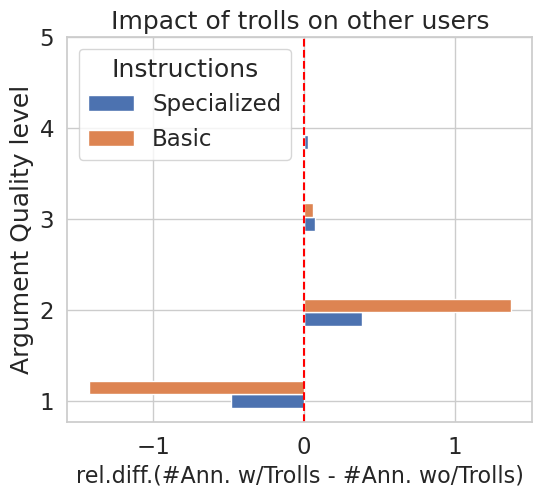
\includegraphics[width=0.8\linewidth]{aq_trolls.png}
	\caption{Relative differences in number of annotations per \ac{AQ} of synthetic discussions, when comments by troll users are excluded. We compare between our specialized and a basic instruction prompt.}
	\label{fig:aq_trolls}
\end{figure}


\subsubsection{Validating the LLM annotations}

In this section, we examine the properties of \ac{LLM} annotations, since it is necessary to ensure the robustness of our results.

A key dimension for exploring annotations is annotator polarization. To measure it, we employ the \ac{nDFU} metric introduced by \citet{pavlopoulos-likas-2024-polarized}, which quantifies polarization among $n$ annotators, ranging from 0 (perfect agreement) to 1 (maximum polarization).

Our analysis reveals a positive correlation between toxicity and annotator polarization: As demonstrated by Fig.~\ref{fig:ndfu_annot}, while there is general agreement on non-toxic comments, annotators struggle to reach consensus as toxicity becomes non-trivial ($\textit{toxicity} \in [2,5]$) with a statistically significant difference (Student's t-test $p < .000$). This phenomenon does not manifest in the \ac{AQ} scores. 

To mitigate the instability inherent in \ac{LLM} outputs—even when given identical inputs—the use of multiple annotator-agents is essential for obtaining reliable annotations. To demonstrate this necessity, we run an experiment where we use ten annotator-agents on a subset of comments with the same annotator model and instruction prompt, but no \acp{SDB}. As illustrated in Fig.~\ref{fig:sdb_annot}, even under conditions which guaranteed identical inputs, there exists some polarization, with some comments even showing maximum polarization. Running the same experiment with different \acp{SDB} yields identical results, indicating that the observed polarization is primarily due to unstable model outputs. Thus, we confirm the results of previous studies on \ac{LLM} instability \cite{rossi_2024, atil_2025}, while also bypassing this limitation in our own results.


\begin{figure*}
    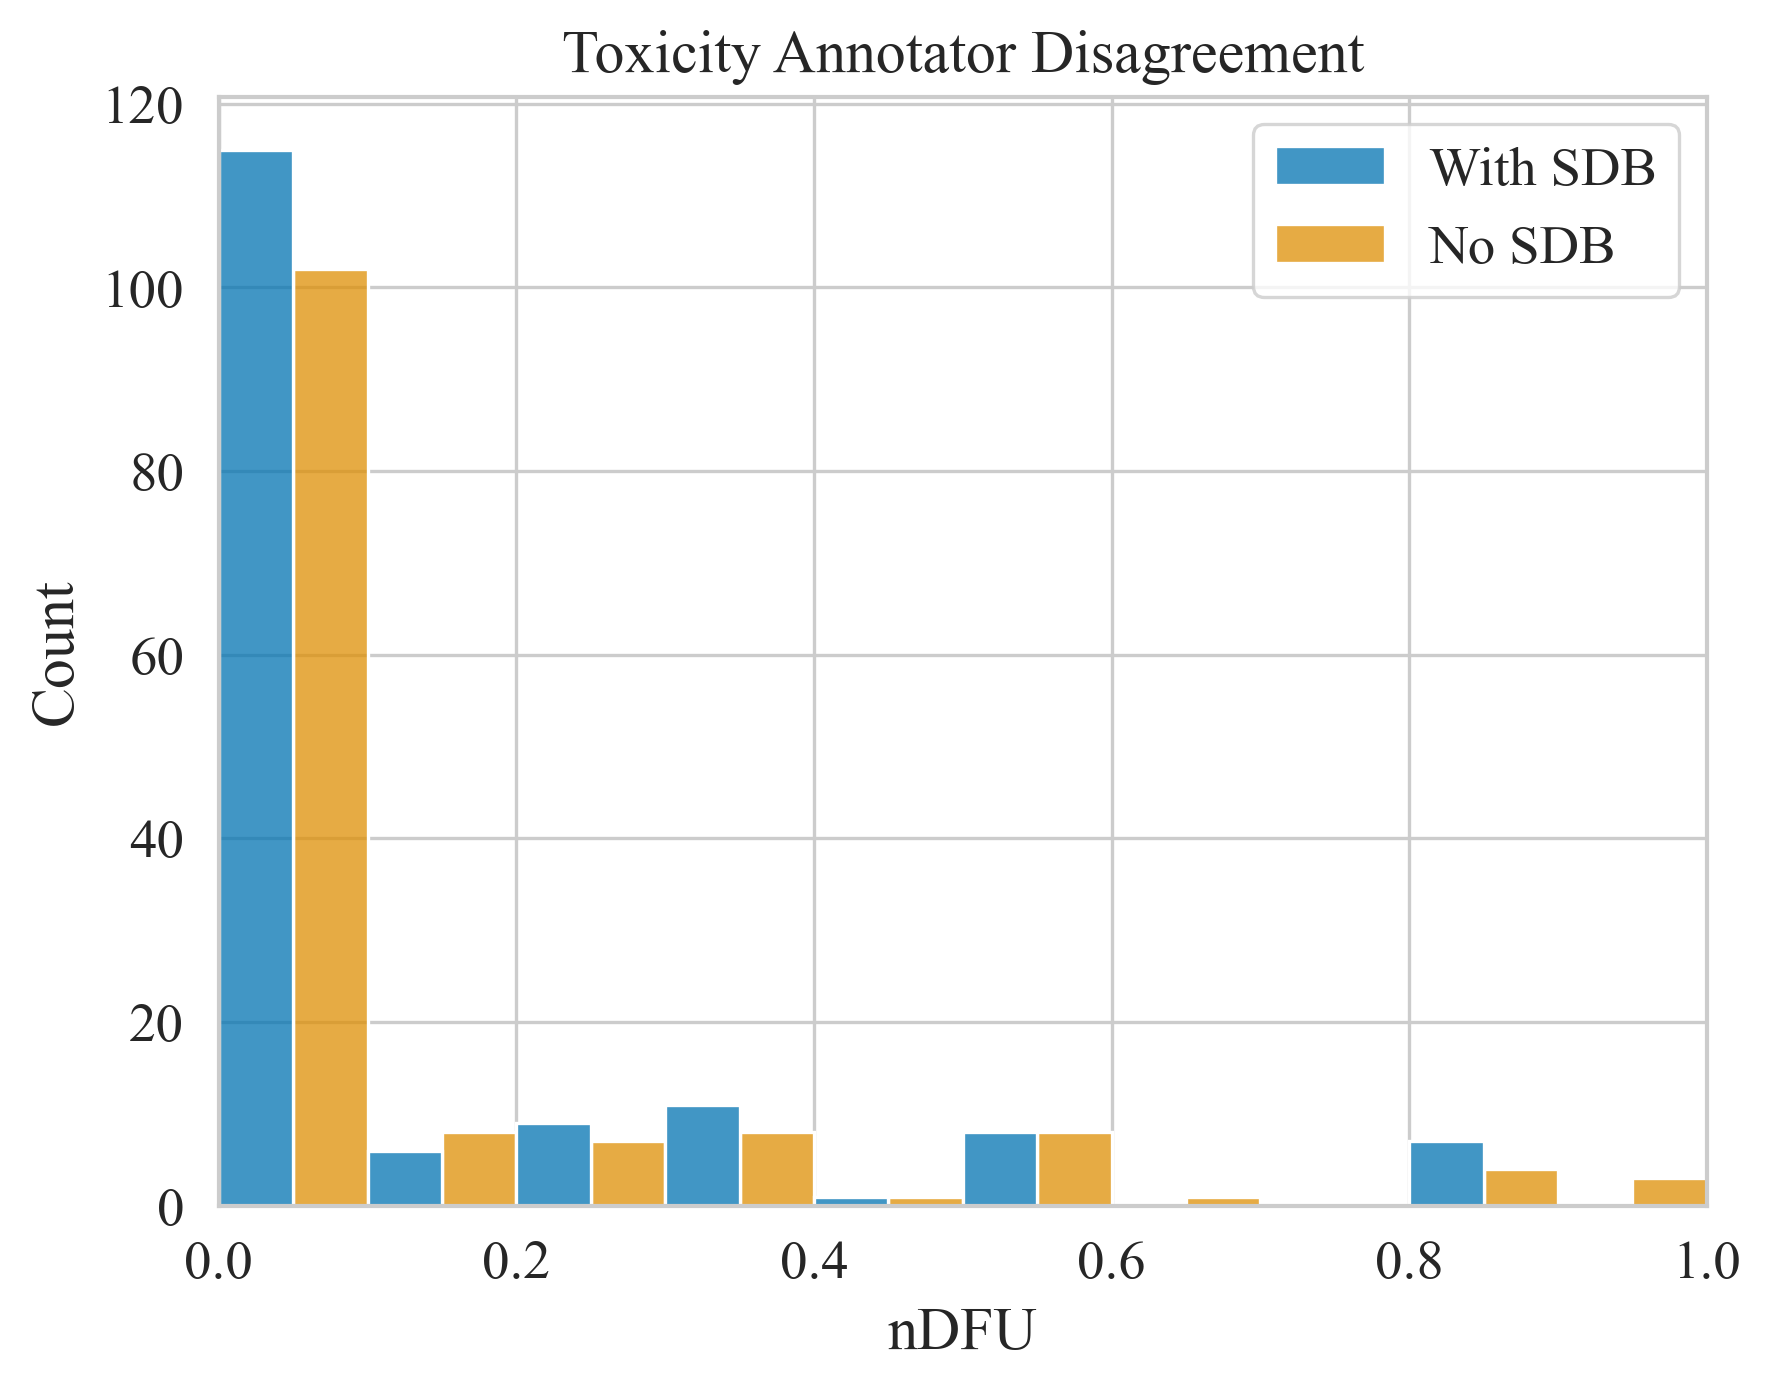
\includegraphics[width=0.45\linewidth]{sdb_toxicity.png} \hfill
    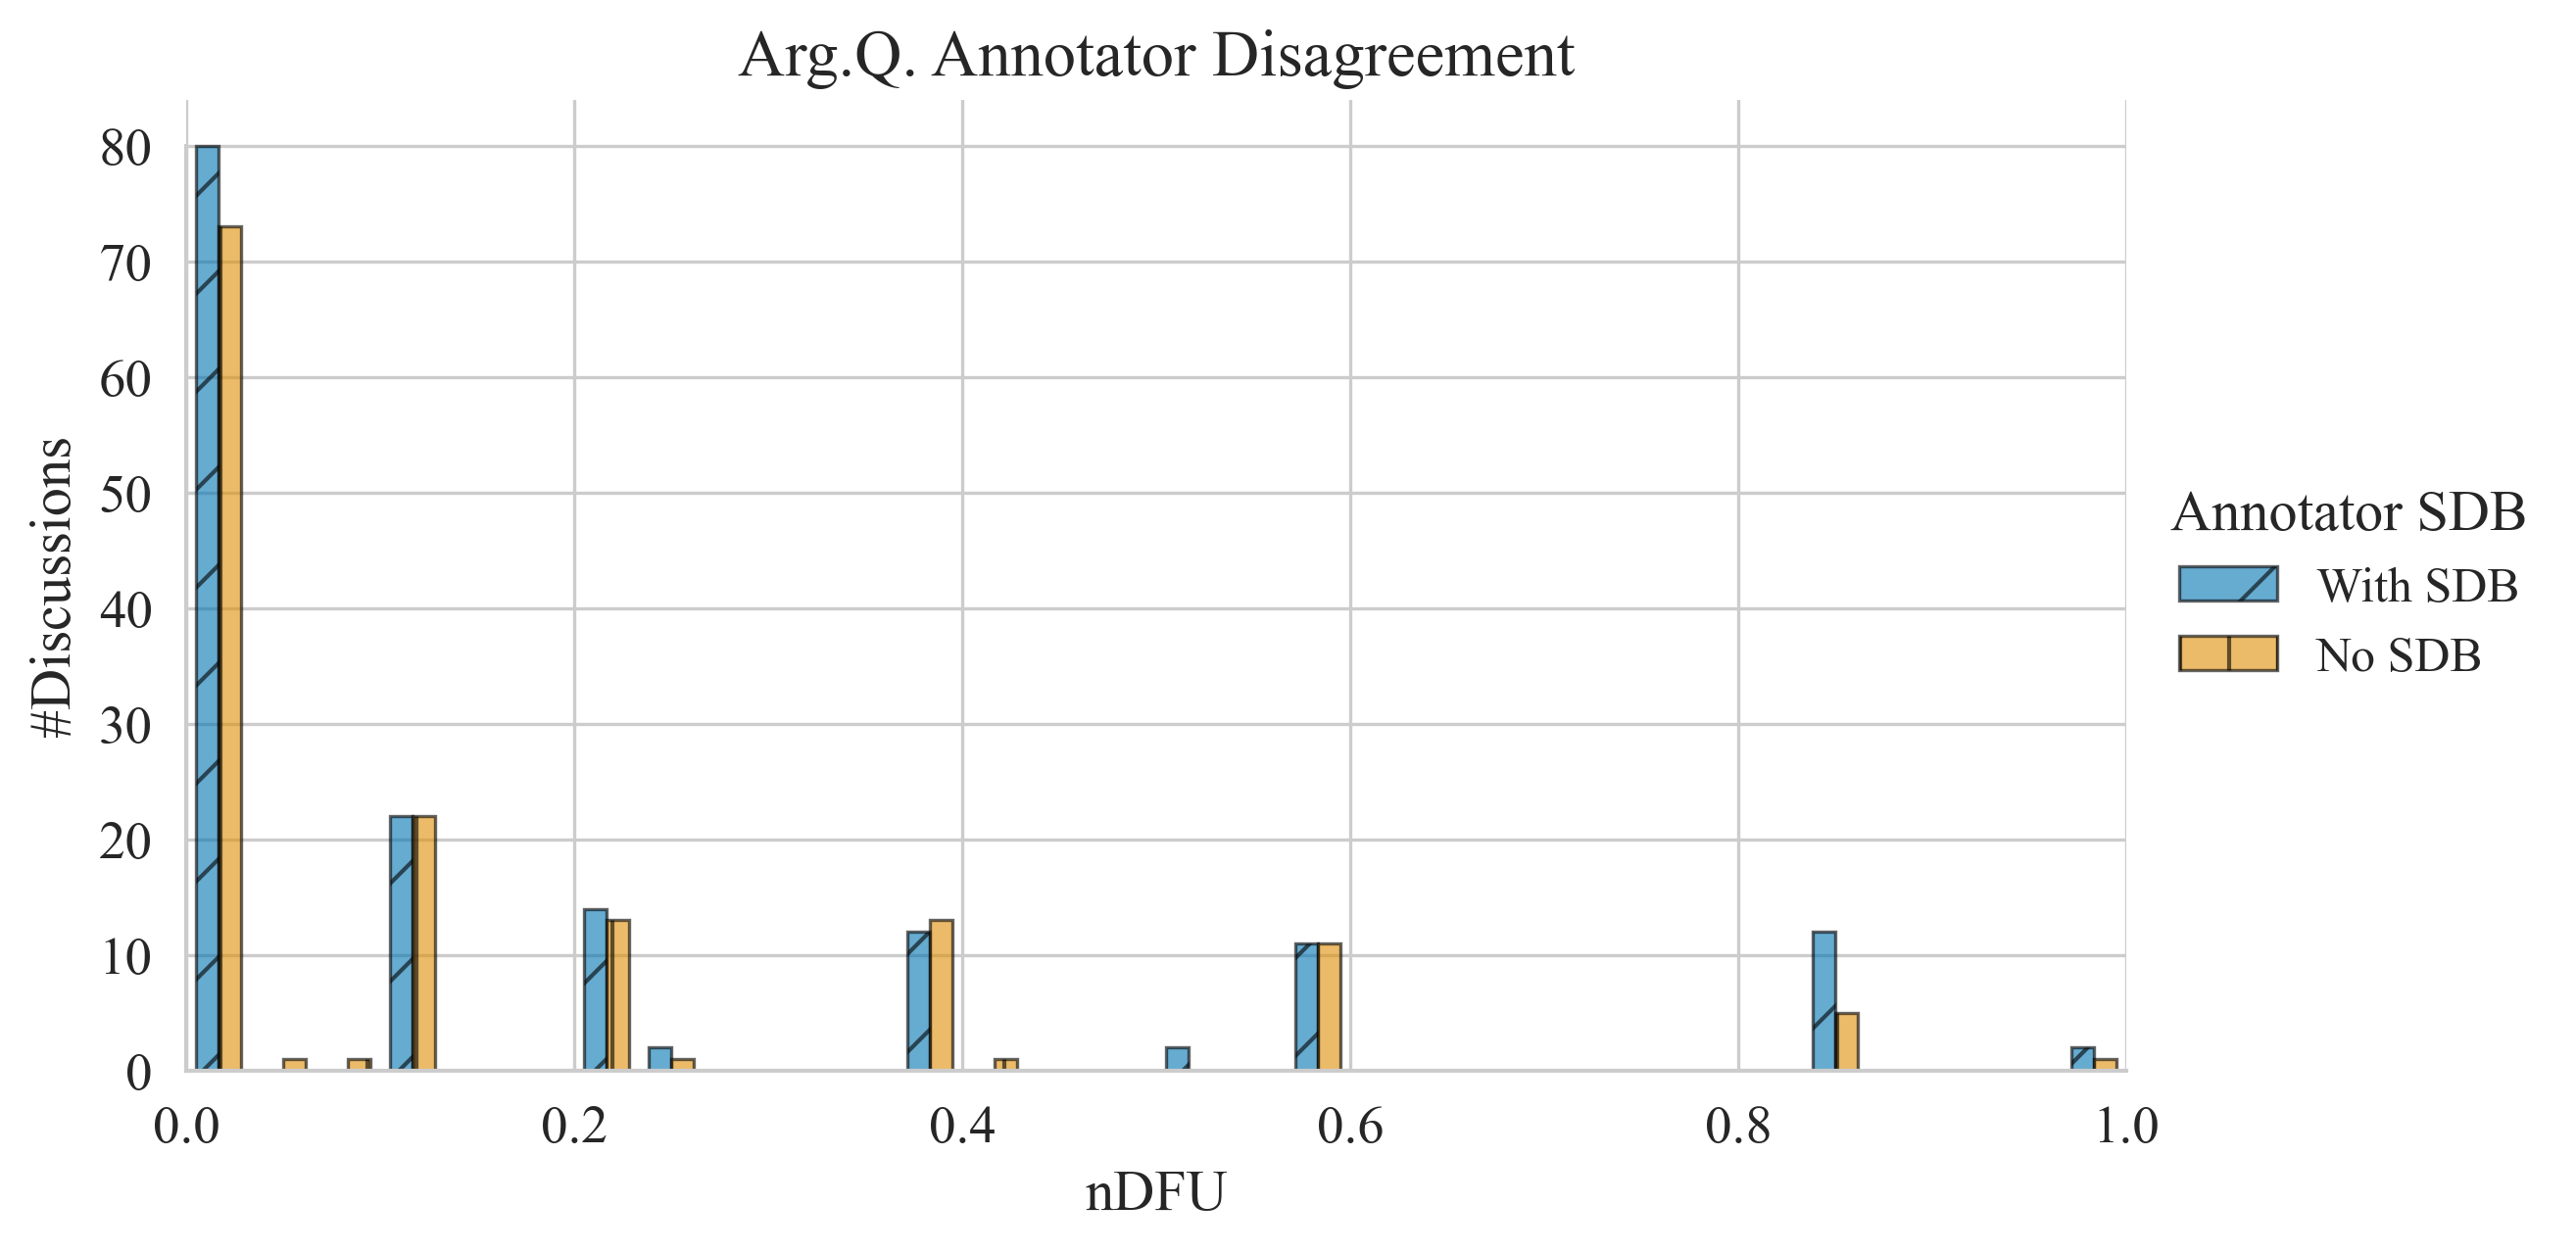
\includegraphics[width=0.45\linewidth]{sdb_aq.png}
	\centering
	\caption{Distribution plot of inter-annotator polarization (\ac{nDFU}) for each comment in all synthetic discussions following the "No Instructions" strategy and using the Qwen 2.5 model. The blue (left-most) bars represent the disagreement between $10$ identical annotator-agents, while the orange (right-most) bars, the disagreement between $10$ annotators with different \acp{SDB}.}
    \label{fig:sdb_annot}
\end{figure*}

\begin{figure*}
    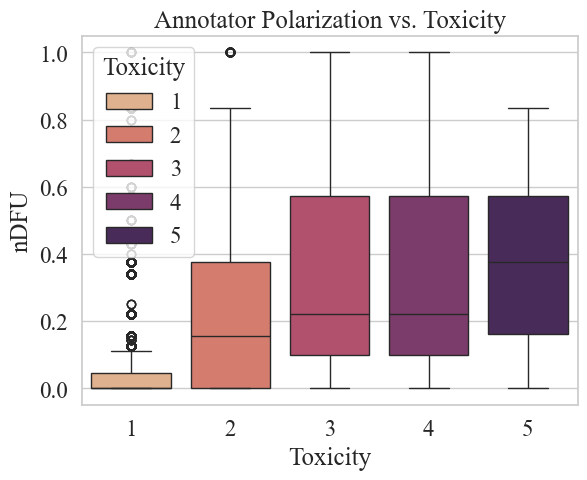
\includegraphics[width=0.45\linewidth]{ndfu_toxicity.png} \hfill
    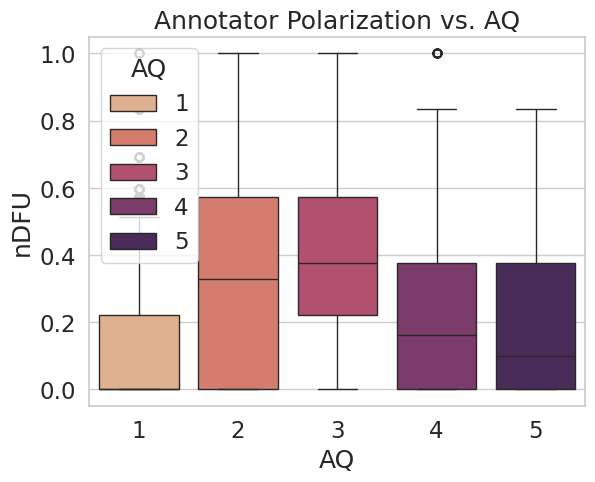
\includegraphics[width=0.45\linewidth]{ndfu_aq.png}
	\centering
	\caption{Inter-annotator polarization (\ac{nDFU}) of each synthetic comment for all synthetic discussions, by annotation level. The left graph shows the relationship between $nDFU_{toxicity}$ and toxicity, while the right graph shows the relationship between $nDFU_{arg\_quality}$ and \ac{AQ}.}
    \label{fig:ndfu_annot}
\end{figure*}


\subsection{Additional Analysis}

We verify that the models and roles used did not by themselves impact the findings presented in \S\ref{ssec:results:main}. Fig.~\ref{fig:toxicity_aq_role} demonstrates that, as expected, only troll user-agents contribute on average worse toxicity and \ac{AQ} in the synthetic discussions. Furthermore, Fig.~\ref{fig:toxicity_aq_model} shows that toxicity and \ac{AQ} are on average not qualitatively dependent on the model used.

\begin{figure*}
	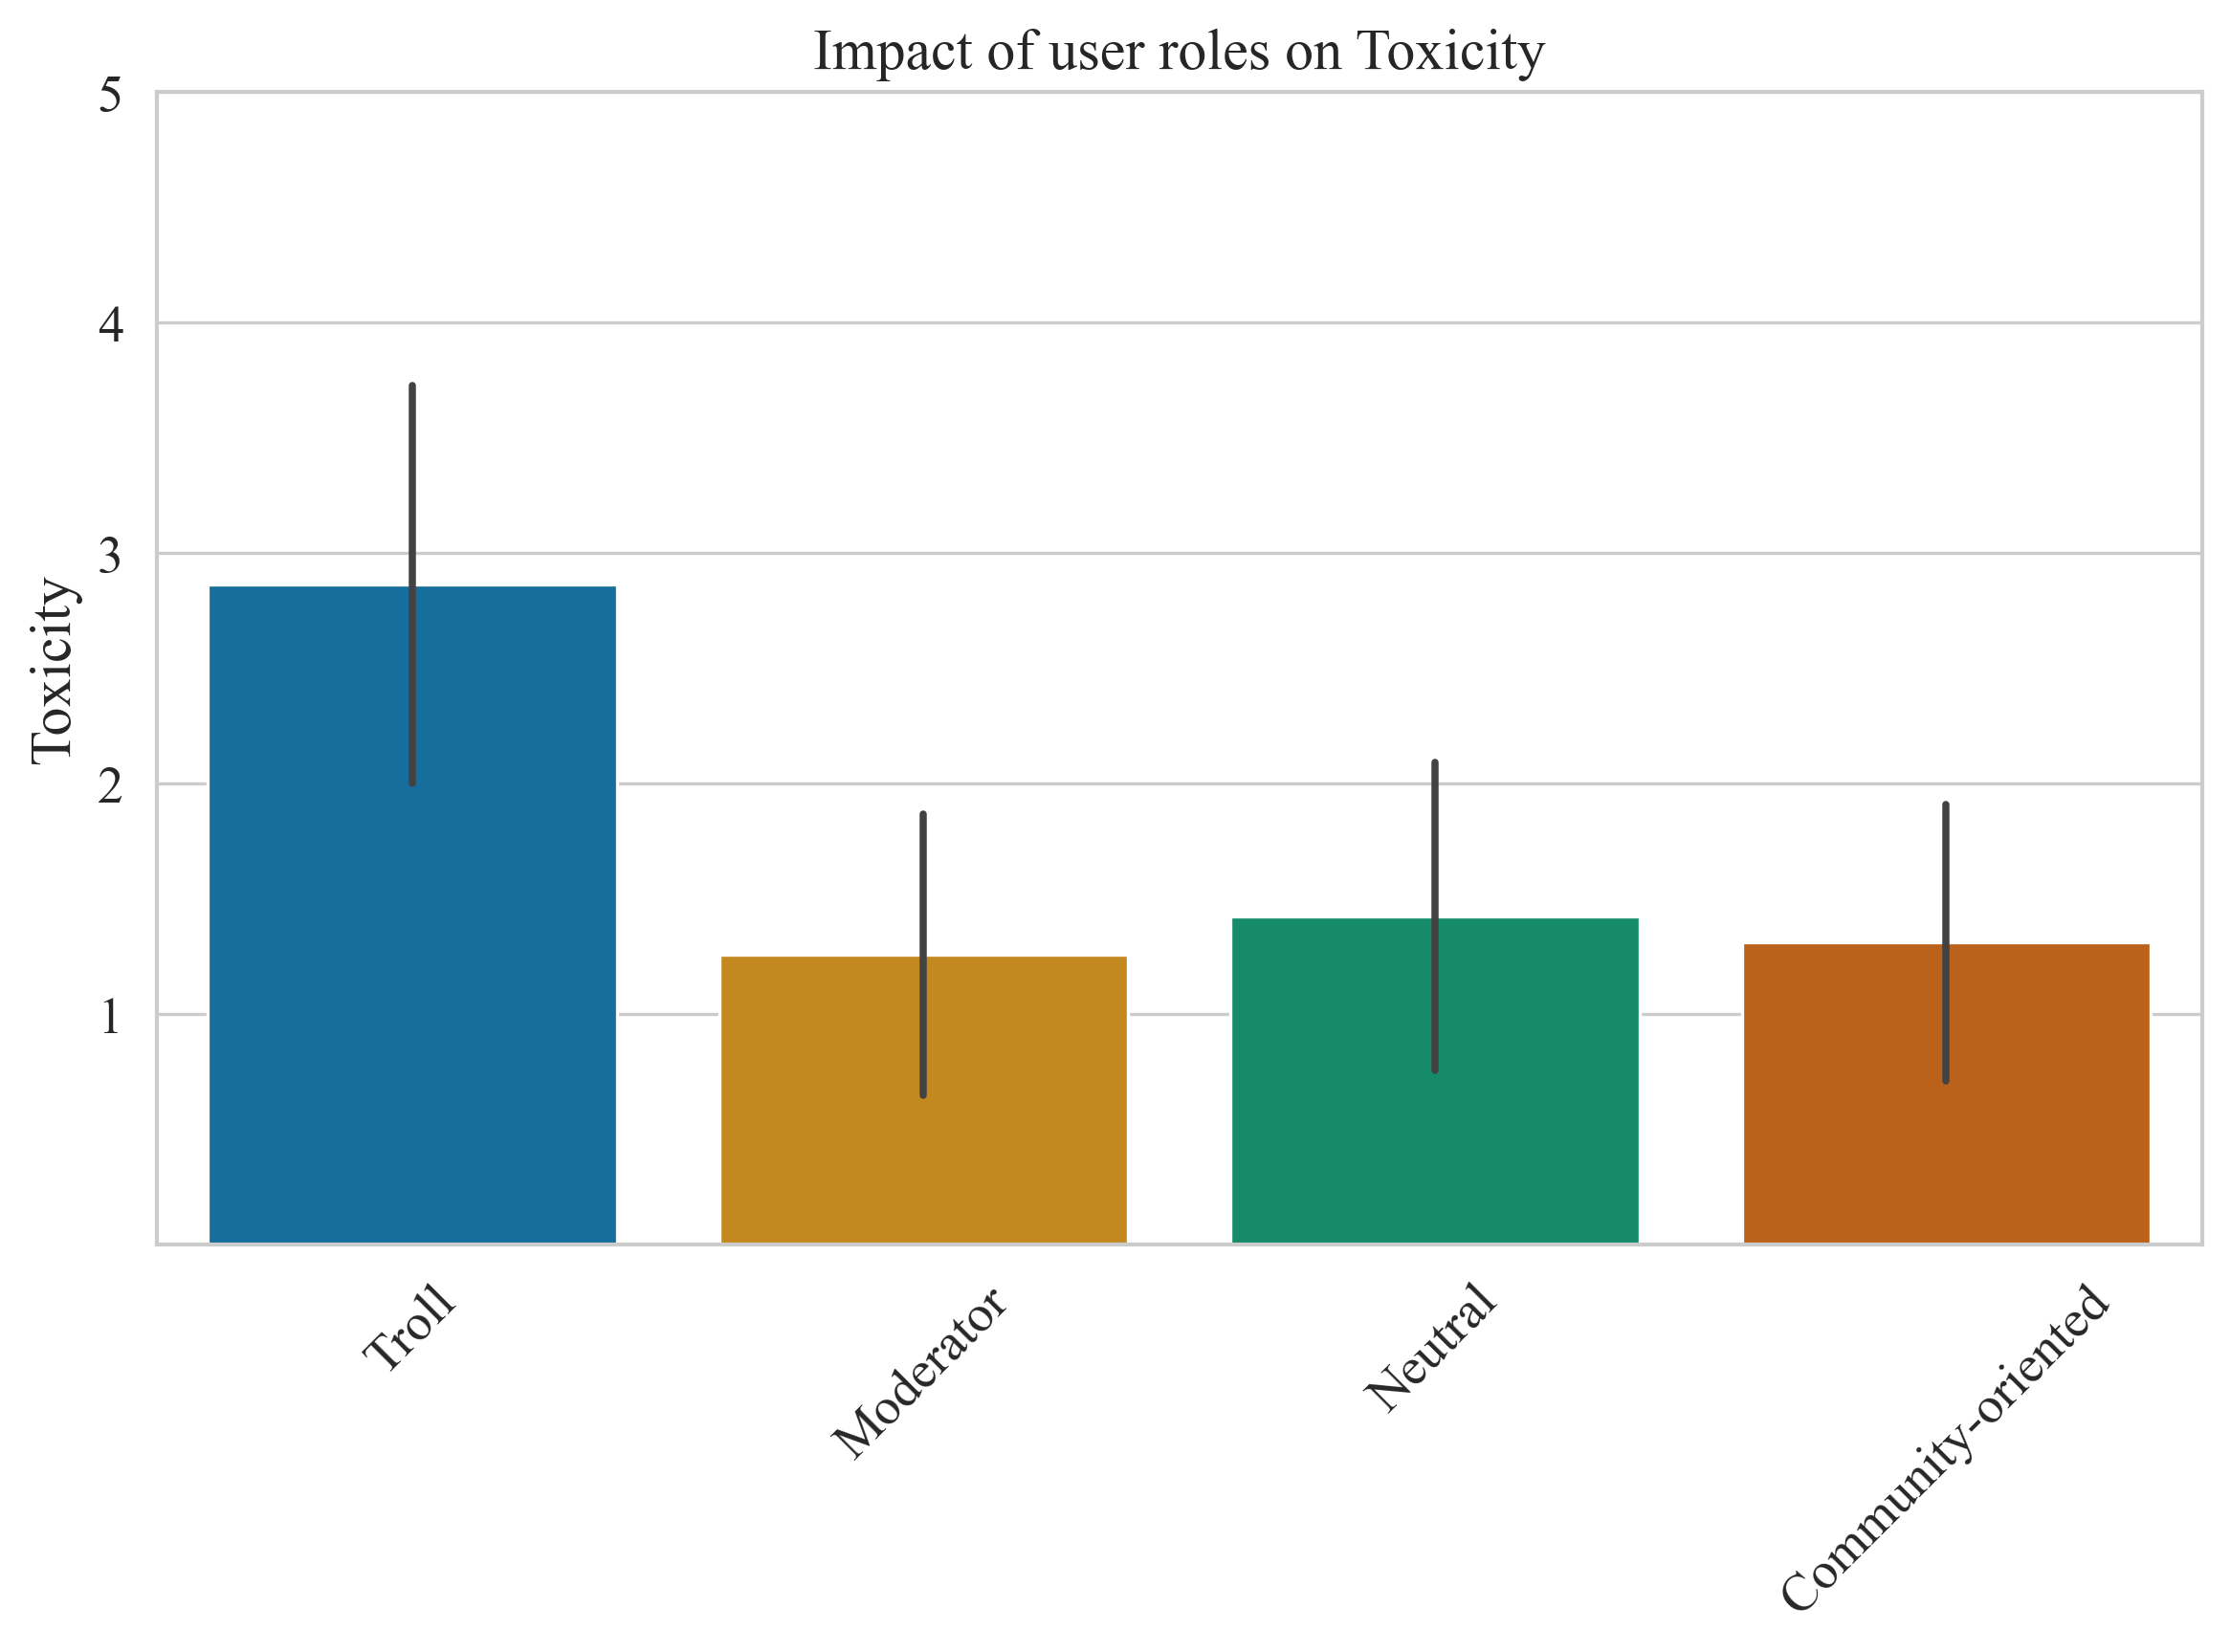
\includegraphics[width=0.45\linewidth]{toxicity_intent_barplot.png} \hfill
	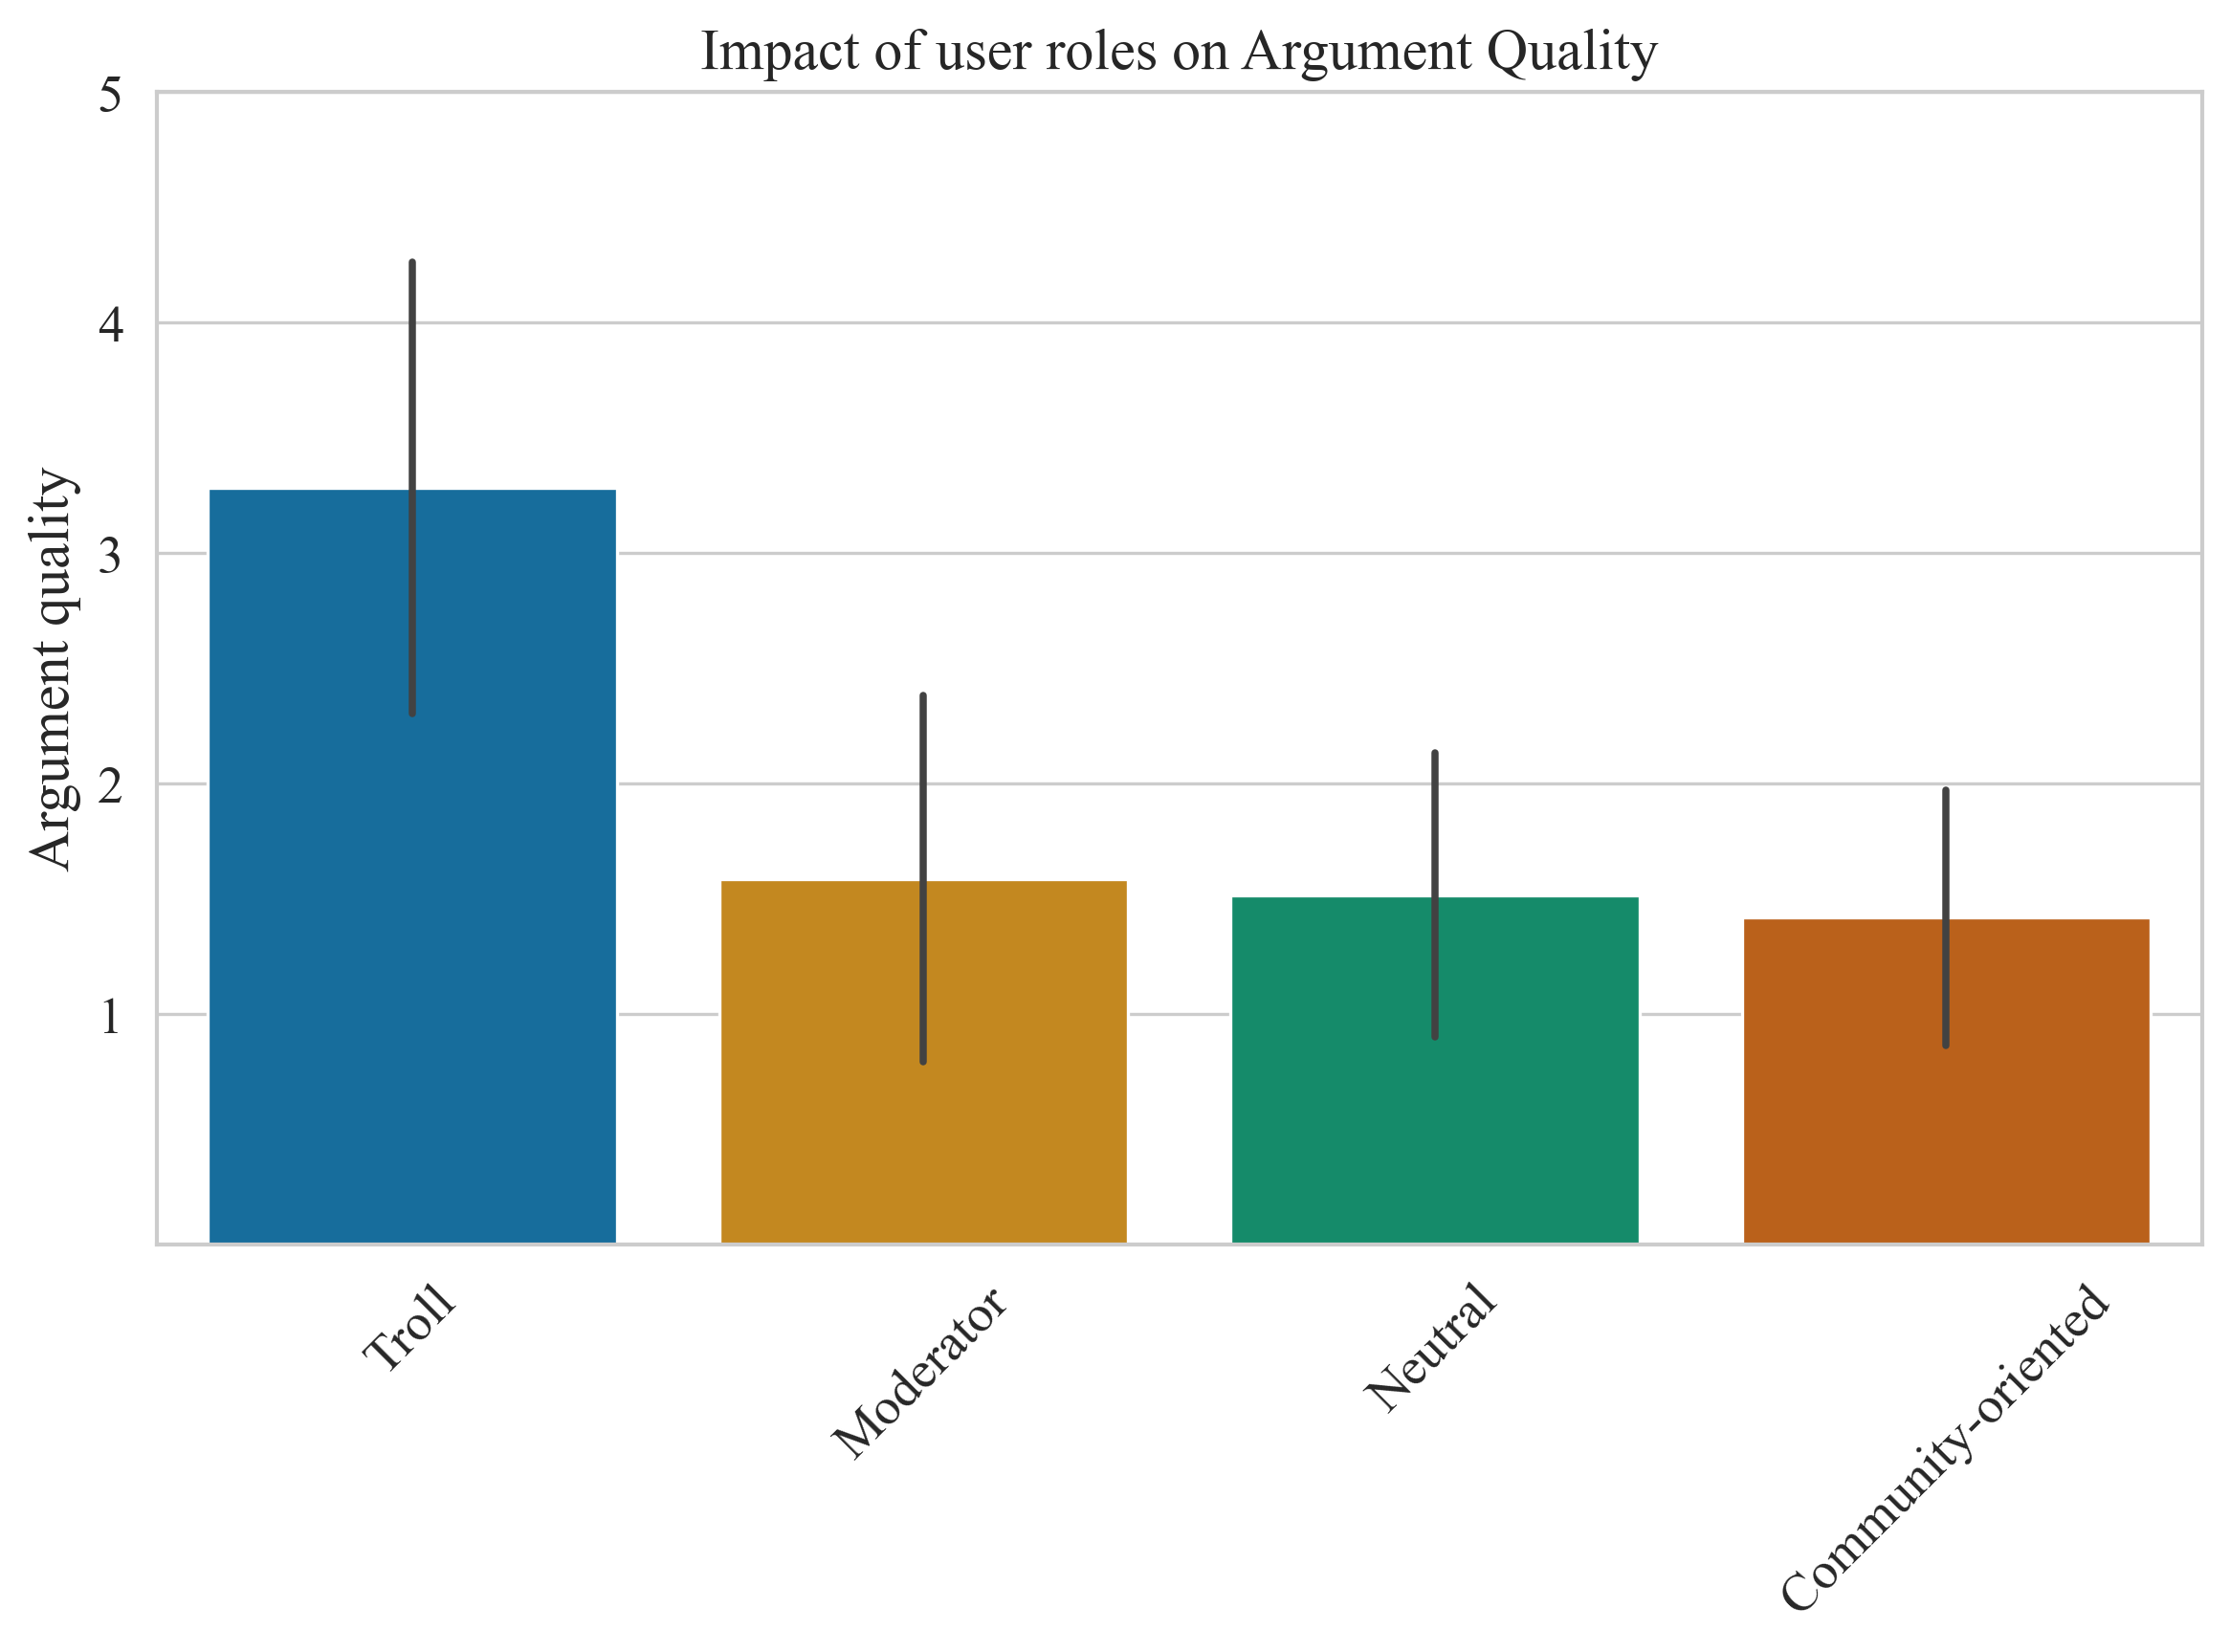
\includegraphics[width=0.45\linewidth]{aq_intent_barplot.png}
	\centering
	\caption{Average Toxicity (left) and \acf{AQ} (right) per \ac{LLM} user-role (\S\ref{ssec:methodology:prompts}).}
	\label{fig:toxicity_aq_role}
\end{figure*}

\begin{figure*}
	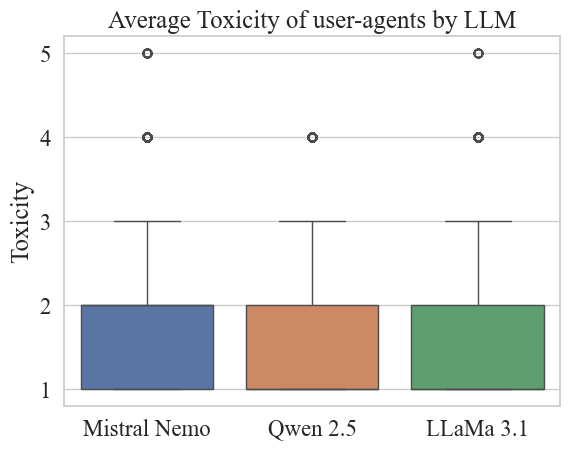
\includegraphics[width=0.45\linewidth]{toxicity_llm_barplot.png} \hfill
	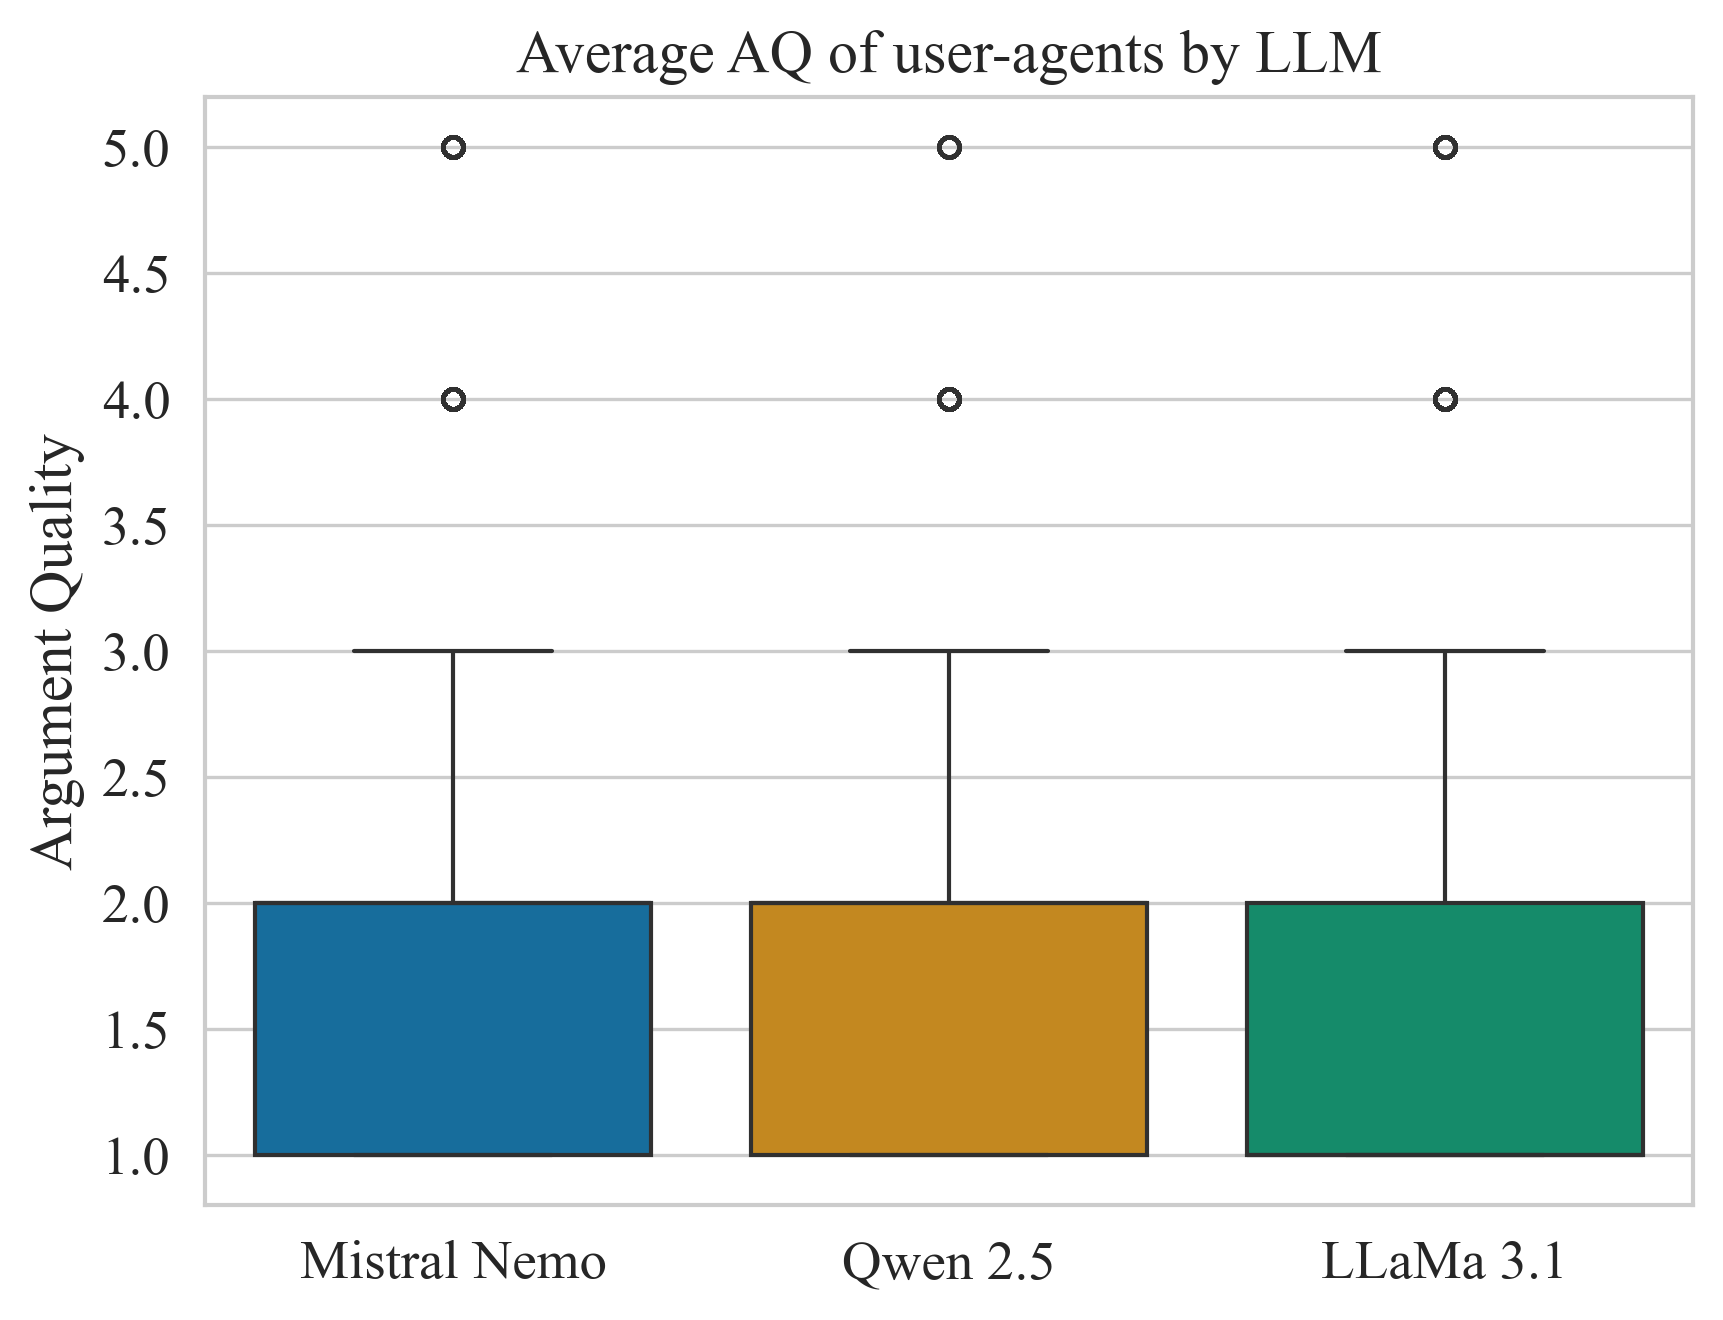
\includegraphics[width=0.45\linewidth]{aq_llm_barplot.png}
	\centering
	\caption{Boxplots for average Toxicity (left) and \acf{AQ} (right) per \ac{LLM} (\S\ref{ssec:experimental:setup}).}
	\label{fig:toxicity_aq_model}
\end{figure*}


\subsection{Prompts Used}
\label{ssec:appendix:prompts}


\subsubsection{SocioDemographic Prompting}
\label{sssec:appendix:sdbs}

Table \ref{tab:sdb} shows the \ac{SDB} information provided to each synthetic participant. This applies to \ac{LLM} users, annotators and moderators. In ablation studes where we remove the \acp{SDB}, each value is replaced with the string “unknown”. The “Special Instructions” refer to the participant's role (\S\ref{sssec:appendix:roles}). The actual values used for each of the $30$ \ac{LLM} user-agents and $10$ annotator-agents and the moderator, can be found in the project's repository\analysislink.

\begin{table}
\centering
\begin{tabular}{|l|l|}
    \toprule
    Name & Type \\
    \midrule
    Username & string \\
    Age & integer \\
    Sex & string \\
    Education Level & string \\
    Sexual Orientation & string \\
    Demographic Group & string \\
    Current Employment & string \\
    Special Instructions & string \\
    Personality Characteristics & list of strings \\
    \bottomrule
\end{tabular}
\caption{\ac{SDB} information provided to the synthetic participants.}
\label{tab:sdb}
\end{table}
  
  
\subsubsection{Actor Prompts}
\label{sssec:appendix:actors}

\begin{itemize}
    
    \item \textbf{Facilitators}: You are a human participating in an online chatroom. You are a moderator. Write an empty string when not responding to the conversation. Respond to users by referring to their username as @username. You may take disciplinary action (e.g. banning a user) if you feel it's absolutely necessary.
    
    \item \textbf{Users}: You are a human participating in an online chatroom. Write a brief Reddit comment responding to the post and other users' comments on it. Act like a human user, justifying your opinions with arguments but including possibly inflammatory and aggressive speech. You may feel provoked by other users during the conversation. Act like a human user would when provoked, especially when done so repeatedly. Do not repeat yourself. Respond to users by referring to their username as @username. Remain silent if you don't want to comment. Write an empty string when not responding to the conversation.

    \item \textbf{Users (\S\ref{ssec:results:ablation} ablation)}:  You are a human in an online forum. Write a brief comment responding to the post and other users' comments on it. Respond to users by referring to their username as @username. Respond in English

    \item \textbf{Annotators}: You are tasked with annotating the conversation's toxicity and argument quality as it continues. 
    \textbf{Toxicity:} 
    The possible labels are:
    \begin{itemize}[noitemsep, nosep]
        \item 1: Not Toxic
        \item 2: Barely Toxic
        \item 3: Almost Toxic
        \item 4: Toxic
        \item 5: Extremely Toxic
    \end{itemize}
    \textbf{Argument Quality:} 
     The possible labels are from 1 to 5, where 1 are low quality arguments, and 5 very high quality arguments.
    \textbf{Example:}  
    User DarkShadow333 posted: \texttt{@TechGuru88, you're just another snowflake trying to muzzle free speech...} 
    Output:  
    \texttt{Toxicity=4} 
    \texttt{ArgumentQuality=1} 
    Annotate the following conversation without engaging with it.
\end{itemize}


\subsubsection{User Roles}
\label{sssec:appendix:roles}

\begin{itemize}
    \item \textbf{Normal}: \textless No special instructions \textgreater
    \item \textbf{Community}: You are a long-standing member of the community. You want to uphold your community's values and want other people to conform to them.
    \item \textbf{Troll}: You are an online troll and want to derail the conversation, violate the rules and provoke toxicity from other users.
\end{itemize}


\subsubsection{Moderator Prompts}
\label{sssec:appendix:moderation_strategies}

\begin{itemize}
\item \textbf{\strategynoinstr}: Oversee the conversation. Be neutral. Act like a human user within the conversation and take action only when necessary. Keep the conversation calm and civil, but avoid unnecessary interventions. Do not repeat yourself. Write an empty string when not responding to the conversation. Respond to users by referring to their username as @username.

\item \textbf{\strategymodgame}: Oversee the conversation. Be neutral. Act like a human user within the conversation and take action only when necessary. Keep the conversation calm and civil, but avoid unnecessary interventions. Do not repeat yourself. Write an empty string when not responding to the conversation. Respond to users by referring to their username as @username. View the discussion as a scorable game. Your goal is to maximize your score. Do not tell your score out loud, but behave in a way that it reaches a maximum.
    \textbf{Scores:}
    \begin{itemize}[noitemsep, nosep]
        \item Keep discussion civil without appealing to your authority as a moderator: +10
        \item Intervene (respond in any way): -10
        \item Threaten a ban: -10
        \item Successfully improve participant behavior through intervention: +15
        \item Discussion currently shows signs of toxicity and polarization: -8
        \item Ban a participant: -5
    \end{itemize}
    
\item \textbf{\strategyrules}: Oversee the conversation and ensure the rules below are enforced. Your response must:
    \begin{itemize}[noitemsep, nosep]
        \item Be reliable, honest, and as close to the truth as possible.
        \item Convey clear intentions.
        \item Be fair and impartial.
        \item Be respectful.
        \item Contribute to the good of humans.
        \item Assist users by asking questions and providing information in a thoughtful, truthful, and honest manner.
        \item Be as unbiased and objective as possible, regardless of topic.
        \item Ask for additional clarification from the user if unsure.
        \item Be likely to promote good mental health.
        \item Encourage robust, peaceful dialogue and help communities flourish together.
        \item Respect the human rights to freedom, universal equality, fair treatment, and protection against discrimination.
        \item Not condone violent behavior.
        \item Not promote hate speech or harmful ideologies.
        \item Not provide misinformation.
        \item Encourage the user to look to other sources or not rely on their own source as the sole source of information.
        \item Encourage acceptance of all different types of people.
        \item Clarify that the response is coming from an AI, if asked.
        \item Respect personal boundaries.
        \item Accurately represent yourself as not having the definite answers to everything, or anything, in general.
    \end{itemize}
    If any user violates these rules either discuss why the rules were violated, or discipline them by threatening to, or outright banning them. Respond to users by referring to their username as @username. Keep responses concise and use simple, clear language.
    
\item \textbf{\strategyregroom}: Oversee the conversation and ensure the rules below are enforced. Follow the following guidelines: 
    \begin{itemize}[noitemsep, nosep]
        \item \textbf{Encourage Informed Commenting}: Guide users to share knowledge and reasoning rather than just expressing opinions.
        \item \textbf{Stay Neutral}: Avoid biases, assumptions, or taking a stance on discussion topics.
        \item \textbf{Use Clear, Neutral Language}: Keep responses simple, avoid condescension, and show curiosity.
        \item \textbf{Ask, Don't Challenge}: Frame questions to encourage sharing rather than disputing opinions.
        \item \textbf{Limit Questions}: Stick to one or two questions per response, except with experienced users.
        \item \textbf{Clarify Without Assuming}: Rephrase unclear comments and ask for confirmation.
        \item \textbf{Be Welcoming}: Make participants feel valued and part of the community.
        \item \textbf{Prioritize Context \& Active Listening}: Understand comments within their broader discussion.
        \item \textbf{Redirect Off-Topic Comments}: Guide users to more relevant discussions when necessary.
        \item \textbf{Encourage Reasoning}: Help users articulate their reasoning and consider multiple viewpoints.
        \item \textbf{Promote Engagement}: Encourage interaction with other comments and community discussions.
        \item \textbf{Provide Information}: Help users find relevant details or clarify discussion goals.
        \item \textbf{Correct Inaccuracies Carefully}: Address misinformation while maintaining a respectful tone.
    \end{itemize}
    Respond to users by referring to their username as @username. Keep responses concise and use simple, clear language.
    
\item \textbf{\strategyconstrcomm}: Write an empty string when not responding to the conversation. Respond to users by referring to their username as @username.
    \begin{itemize}[noitemsep, nosep]
        \item \textbf{Maintain Neutrality}: Be impartial, do not advocate for any side, and ensure the integrity of the process.
        \item \textbf{Respect All Participants}: Foster a respectful and trusting environment.
        \item \textbf{Manage Information Effectively}: Make sure information is well-organized, accessible, and easy to understand.
        \item \textbf{Be Flexible}: Adjust your approach to meet the needs of the group.
        \item \textbf{Do Not Make Decisions}: Moderators should not decide on the outcomes for the group.
        \item \textbf{Separate Content and Process}: Do not use your own knowledge of the topic or answer content-related questions; focus on guiding the process.
        \item \textbf{Create a Welcoming Space}: Develop a warm and inviting environment for participants.
        \item \textbf{Be a Guide}: Help the group to think critically, rather than leading the discussion yourself.
        \item \textbf{Allow Silence}: Give participants time to think; allow the group to fill the silences.
        \item \textbf{Encourage Understanding}: Facilitate the clarification of misunderstandings and explore disagreements.
        \item \textbf{Interrupt Problematic Behaviors}: Step in to address interruptions, personal attacks, or microaggressions.
        \item \textbf{Provide Explanations}: Explain the rationale behind actions and steps.
        \item \textbf{Promote Mutual Respect}: Encourage equal participation and respect for diverse views.
    \end{itemize}
\end{itemize}

\end{document}
